\documentclass[]{article}
\usepackage{lmodern}
\usepackage{amssymb,amsmath}
\usepackage{ifxetex,ifluatex}
\usepackage{fixltx2e} % provides \textsubscript
\ifnum 0\ifxetex 1\fi\ifluatex 1\fi=0 % if pdftex
  \usepackage[T1]{fontenc}
  \usepackage[utf8]{inputenc}
\else % if luatex or xelatex
  \ifxetex
    \usepackage{mathspec}
  \else
    \usepackage{fontspec}
  \fi
  \defaultfontfeatures{Ligatures=TeX,Scale=MatchLowercase}
\fi
% use upquote if available, for straight quotes in verbatim environments
\IfFileExists{upquote.sty}{\usepackage{upquote}}{}
% use microtype if available
\IfFileExists{microtype.sty}{%
\usepackage{microtype}
\UseMicrotypeSet[protrusion]{basicmath} % disable protrusion for tt fonts
}{}
\usepackage[margin=1in]{geometry}
\usepackage{hyperref}
\hypersetup{unicode=true,
            pdftitle={PCBs covariance matrix investigation},
            pdfauthor={Xuelong Wang},
            pdfborder={0 0 0},
            breaklinks=true}
\urlstyle{same}  % don't use monospace font for urls
\usepackage{graphicx,grffile}
\makeatletter
\def\maxwidth{\ifdim\Gin@nat@width>\linewidth\linewidth\else\Gin@nat@width\fi}
\def\maxheight{\ifdim\Gin@nat@height>\textheight\textheight\else\Gin@nat@height\fi}
\makeatother
% Scale images if necessary, so that they will not overflow the page
% margins by default, and it is still possible to overwrite the defaults
% using explicit options in \includegraphics[width, height, ...]{}
\setkeys{Gin}{width=\maxwidth,height=\maxheight,keepaspectratio}
\IfFileExists{parskip.sty}{%
\usepackage{parskip}
}{% else
\setlength{\parindent}{0pt}
\setlength{\parskip}{6pt plus 2pt minus 1pt}
}
\setlength{\emergencystretch}{3em}  % prevent overfull lines
\providecommand{\tightlist}{%
  \setlength{\itemsep}{0pt}\setlength{\parskip}{0pt}}
\setcounter{secnumdepth}{5}
% Redefines (sub)paragraphs to behave more like sections
\ifx\paragraph\undefined\else
\let\oldparagraph\paragraph
\renewcommand{\paragraph}[1]{\oldparagraph{#1}\mbox{}}
\fi
\ifx\subparagraph\undefined\else
\let\oldsubparagraph\subparagraph
\renewcommand{\subparagraph}[1]{\oldsubparagraph{#1}\mbox{}}
\fi

%%% Use protect on footnotes to avoid problems with footnotes in titles
\let\rmarkdownfootnote\footnote%
\def\footnote{\protect\rmarkdownfootnote}

%%% Change title format to be more compact
\usepackage{titling}

% Create subtitle command for use in maketitle
\providecommand{\subtitle}[1]{
  \posttitle{
    \begin{center}\large#1\end{center}
    }
}

\setlength{\droptitle}{-2em}

  \title{PCBs covariance matrix investigation}
    \pretitle{\vspace{\droptitle}\centering\huge}
  \posttitle{\par}
    \author{Xuelong Wang}
    \preauthor{\centering\large\emph}
  \postauthor{\par}
      \predate{\centering\large\emph}
  \postdate{\par}
    \date{2019-08-22}

\usepackage{float,amsmath, bbm, siunitx, bm}
\usepackage{pdfpages}
\floatplacement{figure}{H}
\newcommand{\indep}{\rotatebox[origin=c]{90}{$\models$}}

\begin{document}
\maketitle

{
\setcounter{tocdepth}{2}
\tableofcontents
}
\section{Motivation}\label{motivation}

The sample covariates matrix of PCBs is unstructured and dense, so it is
not straightforward to estimate a large, non-spare covariance matrix
directly. One possible solution is to borrow the information from
histrocial data or data from other studies with different responses but
similar covariates. The report is to investigate the covariance matrix
across all the available PCBs data from NHANES from 1999 - 2014. We are
trying to see if there is common structure among all different surveies
or within certain subgroups.

\subsection{Decorrelation using histrocial
data}\label{decorrelation-using-histrocial-data}

\subsubsection{Decorrelation steps}\label{decorrelation-steps}

Let X be the covariates and the
\(\hat{\Sigma}_X = \frac{1}{n-1}(X - \bar{X})^T(X - \bar{X})\). Assume
that there is a matrix A that we could used for decorrelation.

\[
Z = XA \Rightarrow \hat{\Sigma}_Z = \frac{1}{n-1} (Z - \bar{X})^T(Z - \bar{Z}) =  A^T\hat{\Sigma}_XA
\]

\section{PCBs data summary and covariance-correlation
structure}\label{pcbs-data-summary-and-covariance-correlation-structure}

\subsection{1999-2004}\label{section}

There are 3 surveys were conducted during the 6 years. However, based on
the data I collected, the types of PCBs are not extact same accross the
3 surveys. Followings are some facts.

The types of PCBs measured for each survey is

\begin{verbatim}
$`1999`
 [1] "PCB028" "PCB052" "PCB066" "PCB074" "PCB099" "PCB101" "PCB105"
 [8] "PCB118" "PCB128" "PCB138" "PCB146" "PCB153" "PCB156" "PCB157"
[15] "PCB167" "PCB170" "PCB172" "PCB177" "PCB178" "PCB180" "PCB183"
[22] "PCB187"

$`2001`
 [1] "PCB052" "PCB066" "PCB074" "PCB087" "PCB099" "PCB101" "PCB105"
 [8] "PCB110" "PCB118" "PCB128" "PCB138" "PCB146" "PCB149" "PCB151"
[15] "PCB153" "PCB156" "PCB157" "PCB167" "PCB170" "PCB172" "PCB177"
[22] "PCB178" "PCB180" "PCB183" "PCB187" "PCB189" "PCB194" "PCB195"
[29] "PCB196" "PCB199" "PCB206"

$`2003`
 [1] "PCB028" "PCB066" "PCB074" "PCB105" "PCB118" "PCB156" "PCB157"
 [8] "PCB167" "PCB189" "PCB044" "PCB049" "PCB052" "PCB087" "PCB099"
[15] "PCB101" "PCB110" "PCB128" "PCB138" "PCB146" "PCB149" "PCB151"
[22] "PCB153" "PCB170" "PCB172" "PCB177" "PCB178" "PCB180" "PCB183"
[29] "PCB187" "PCB194" "PCB195" "PCB196" "PCB199" "PCB206" "PCB209"
\end{verbatim}

The common PCBs that were measured by each survey is

\begin{verbatim}
 [1] "PCB052" "PCB066" "PCB074" "PCB099" "PCB101" "PCB105" "PCB118"
 [8] "PCB128" "PCB138" "PCB146" "PCB153" "PCB156" "PCB157" "PCB167"
[15] "PCB170" "PCB172" "PCB177" "PCB178" "PCB180" "PCB183" "PCB187"
\end{verbatim}

I will use those 21 PCBs to calculate their covariance matrix.

The total number of PCBs data from 1999-2004 is 7106. After I remove all
the missing data, what I get is total 4873 observations.

Note that I only work on the PCBs measurement without adjustment, but I
used the under the limit adjustment.

\subsubsection{time}\label{time}

Followings are 3 heat-maps of correlation-matrix across the 3 surveys.
In general, they have high correlations among those PCBs. But they do
show some common pattern.

The number of observation across each survey is

\begin{verbatim}
   SDDSRVYR    N
1:        1 1647
2:        2 1435
3:        3 1791
\end{verbatim}

\begin{figure}
\centering
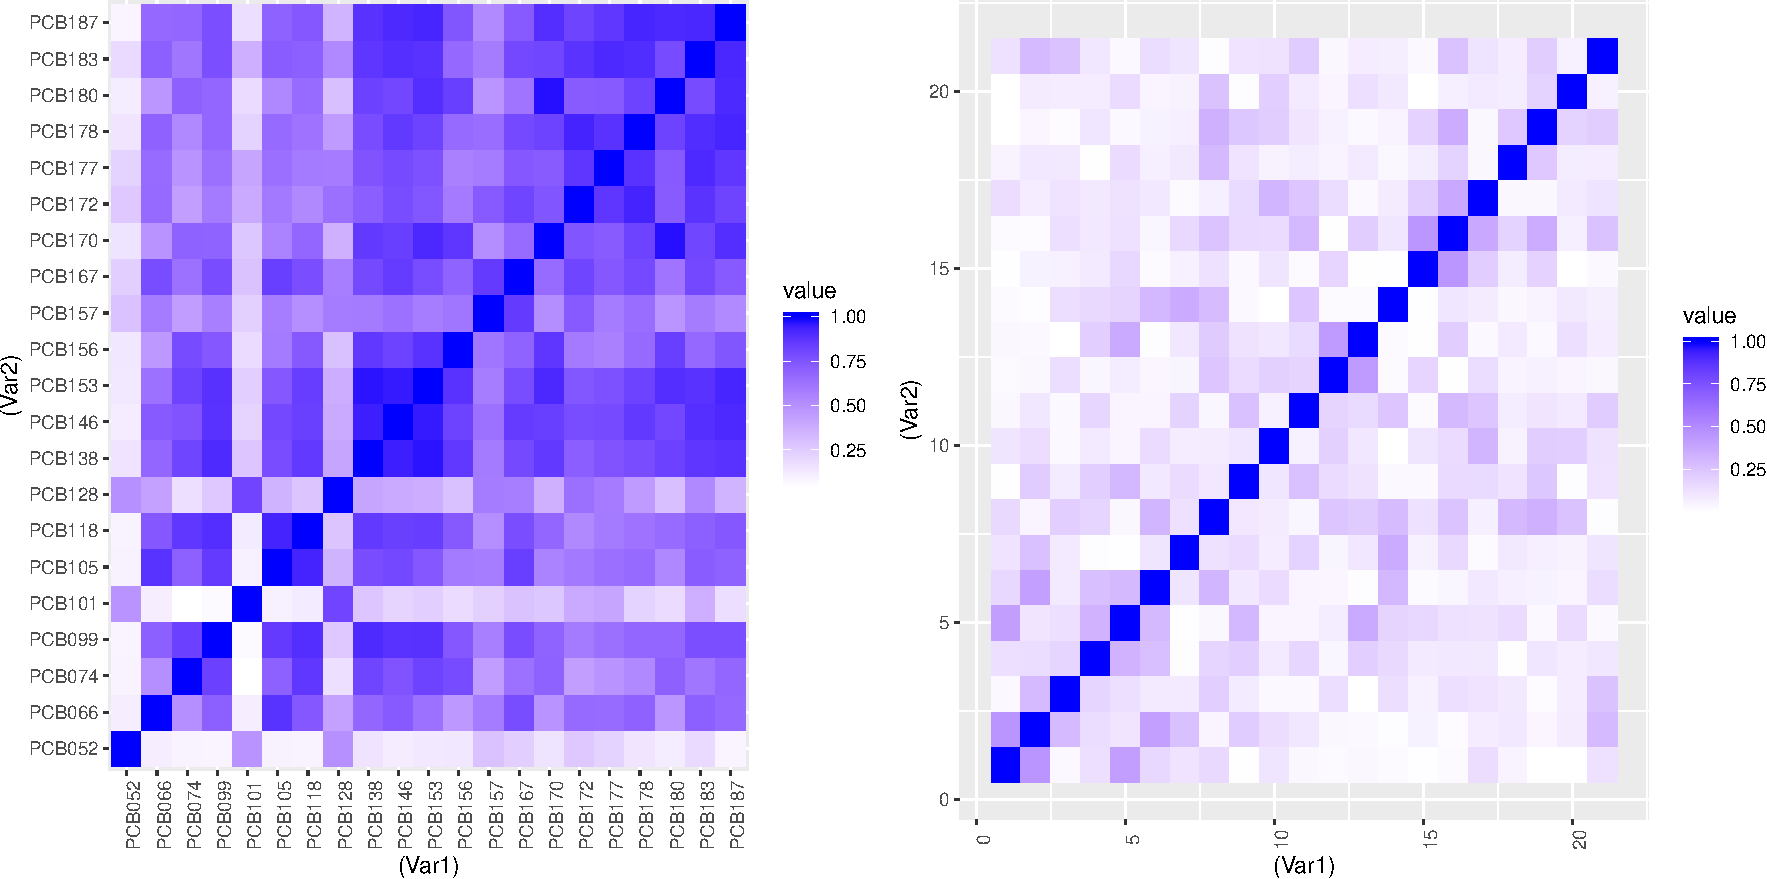
\includegraphics{PCBs_covariance_files/figure-latex/unnamed-chunk-5-1.pdf}
\caption{1999-2000}
\end{figure}

\begin{figure}
\centering
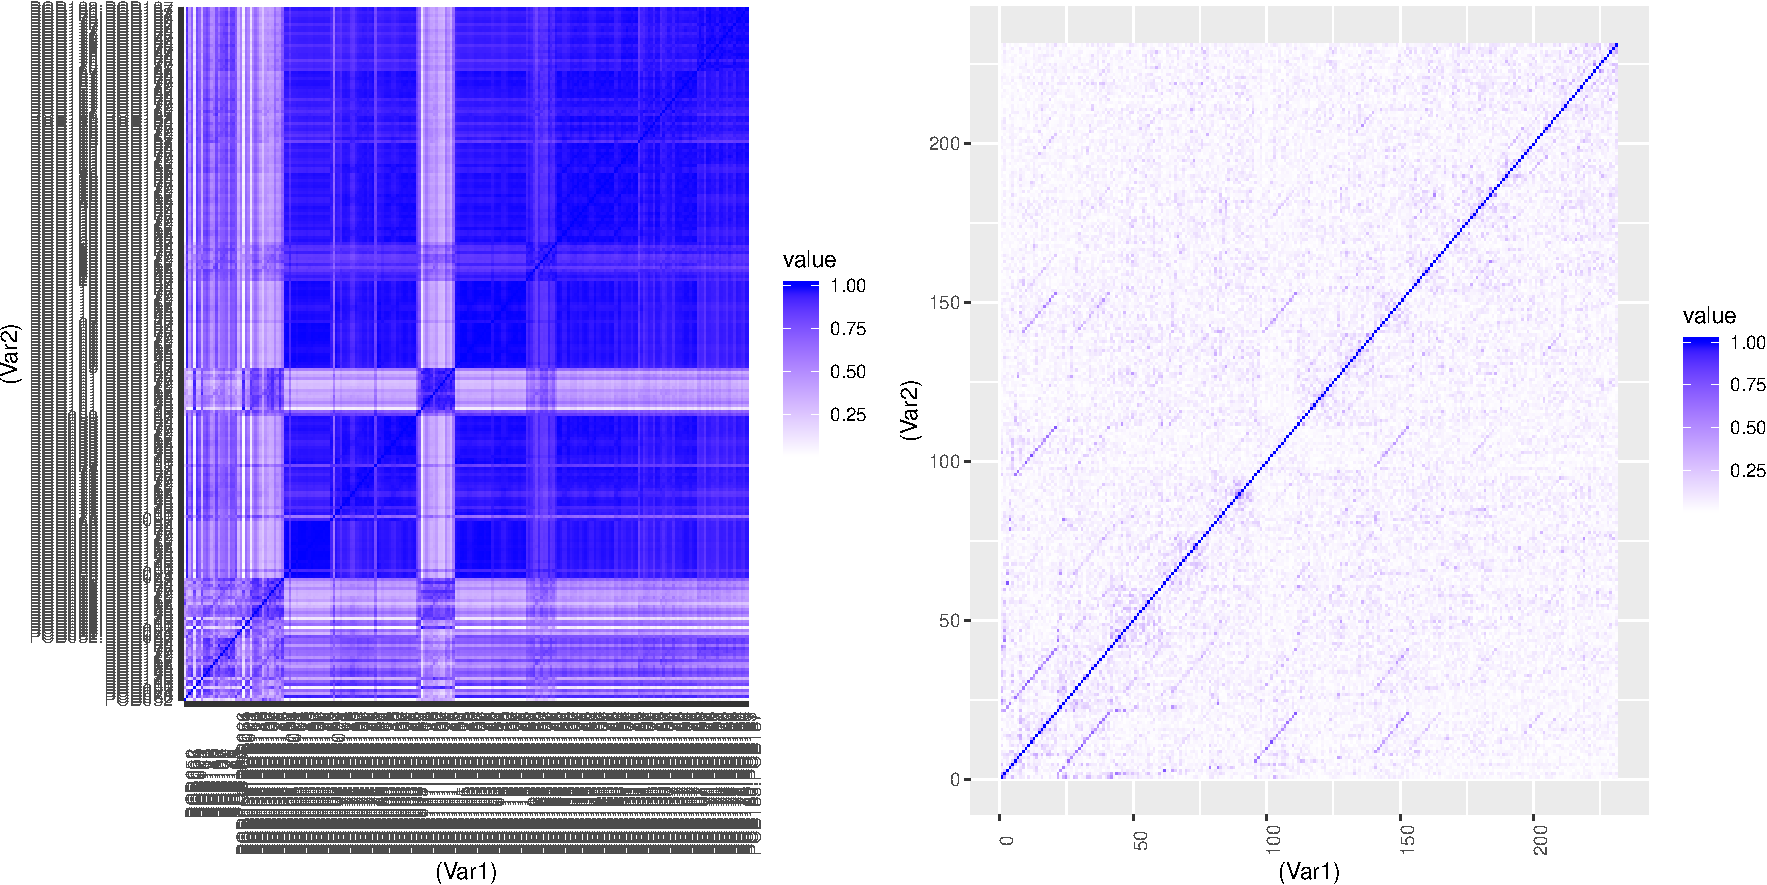
\includegraphics{PCBs_covariance_files/figure-latex/unnamed-chunk-6-1.pdf}
\caption{Combined main and interaction 1999-2000}
\end{figure}

\begin{figure}
\centering
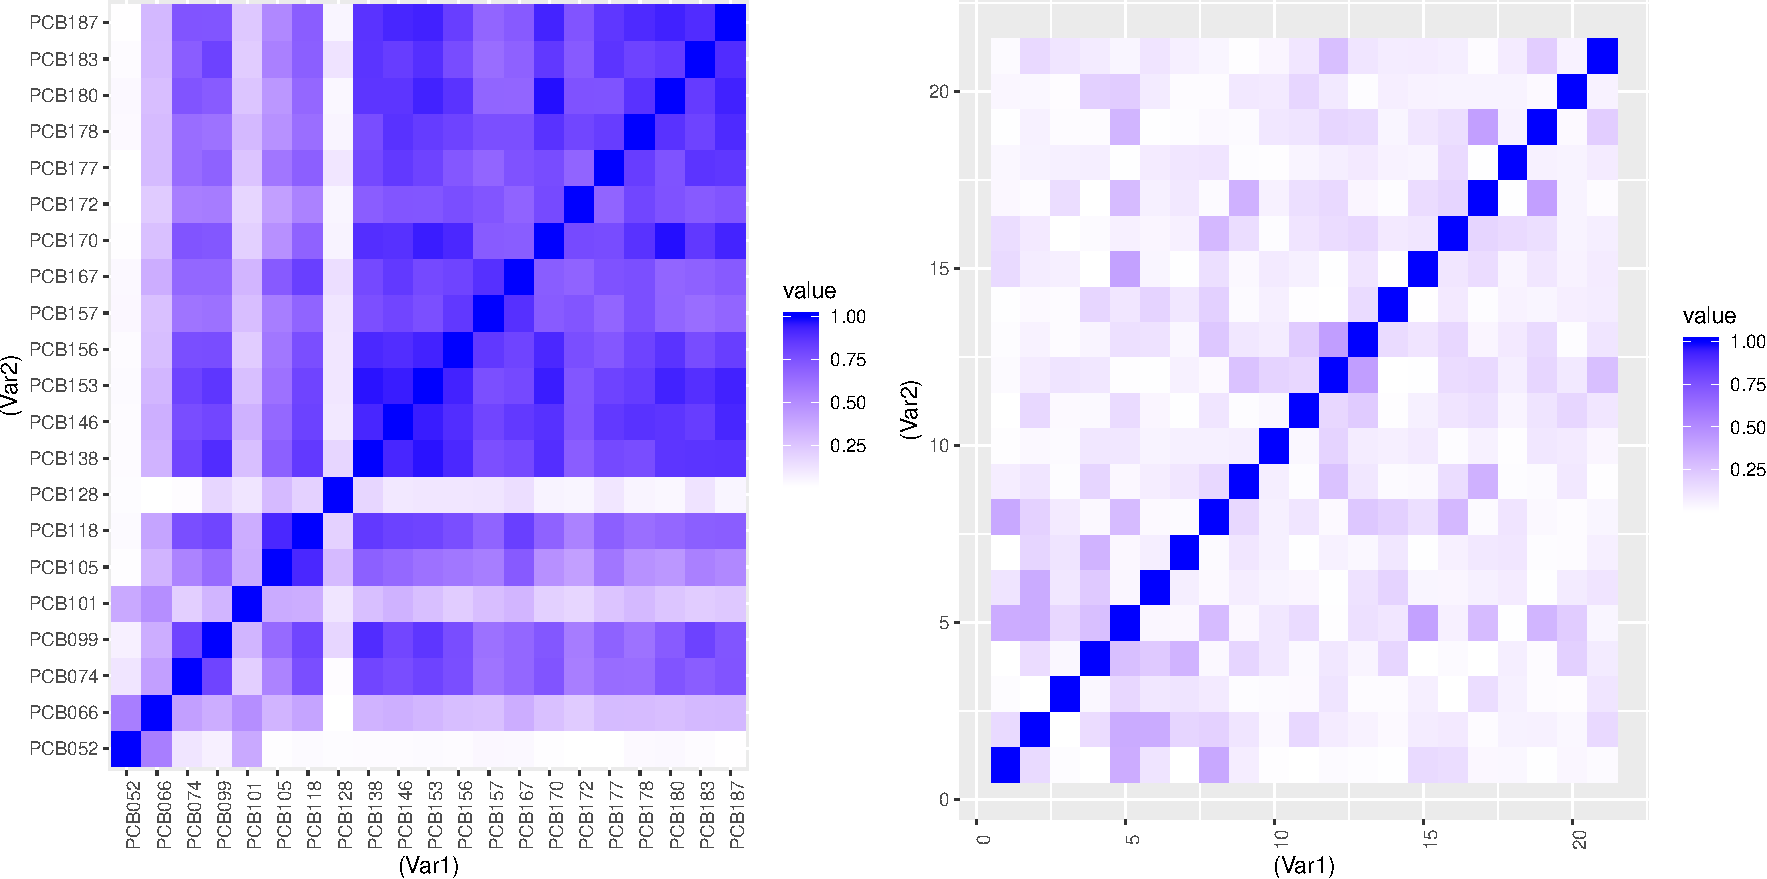
\includegraphics{PCBs_covariance_files/figure-latex/unnamed-chunk-7-1.pdf}
\caption{2001-2002}
\end{figure}

\begin{figure}
\centering
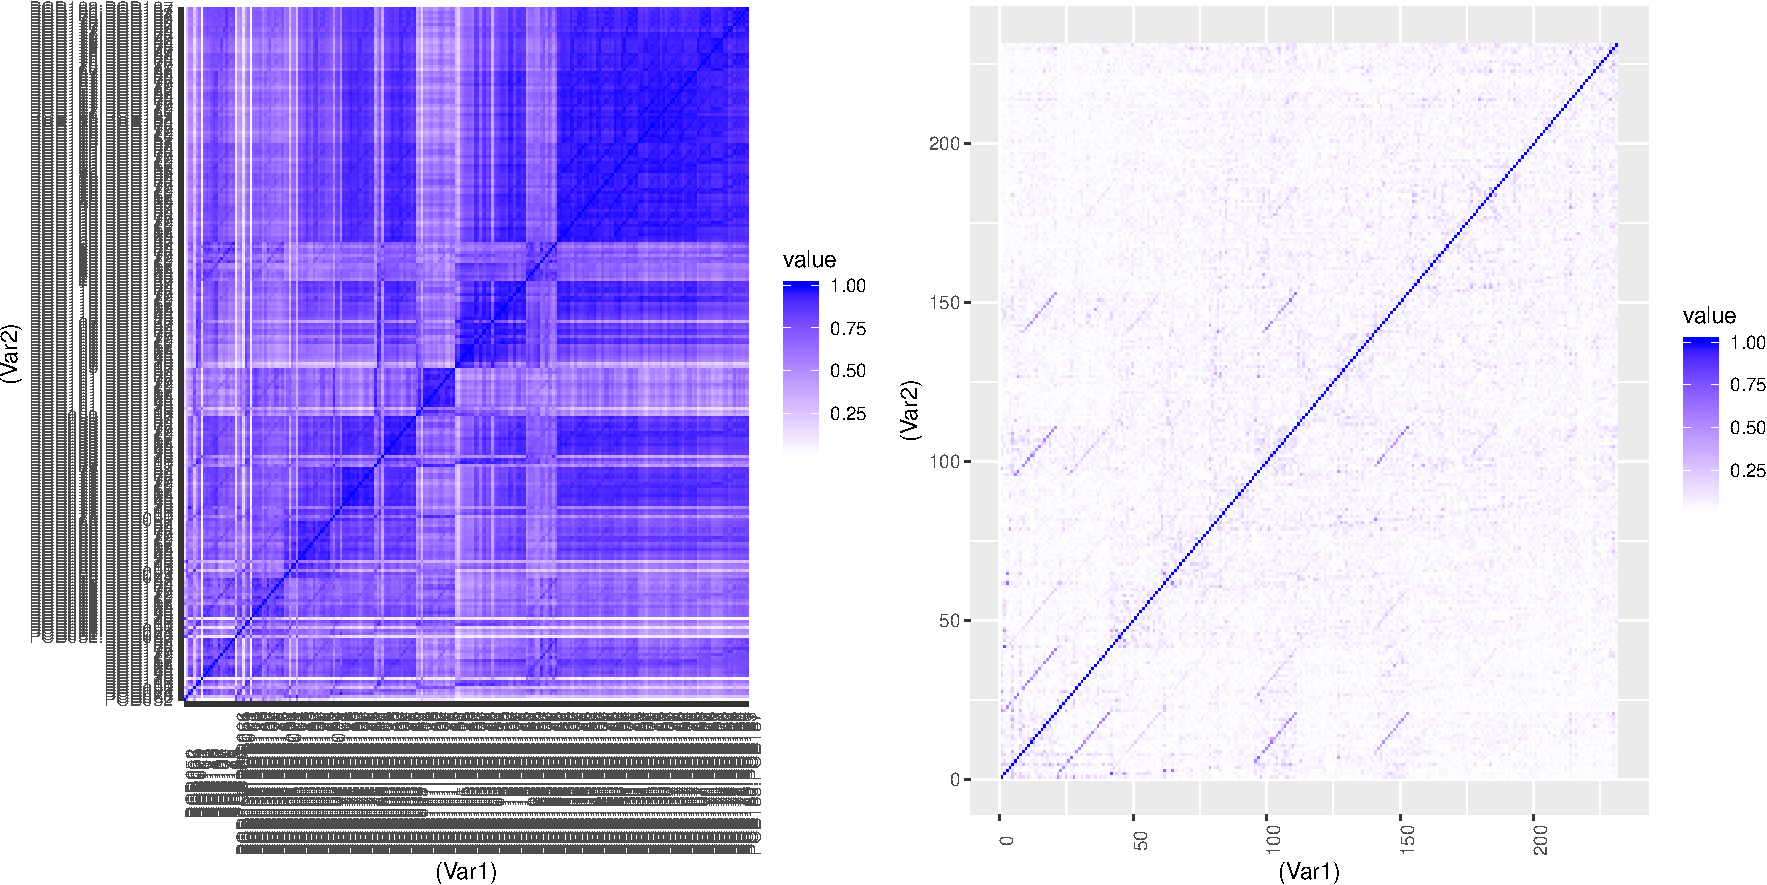
\includegraphics{PCBs_covariance_files/figure-latex/unnamed-chunk-8-1.pdf}
\caption{Combined main and interaction 2001-2002}
\end{figure}

\begin{figure}
\centering
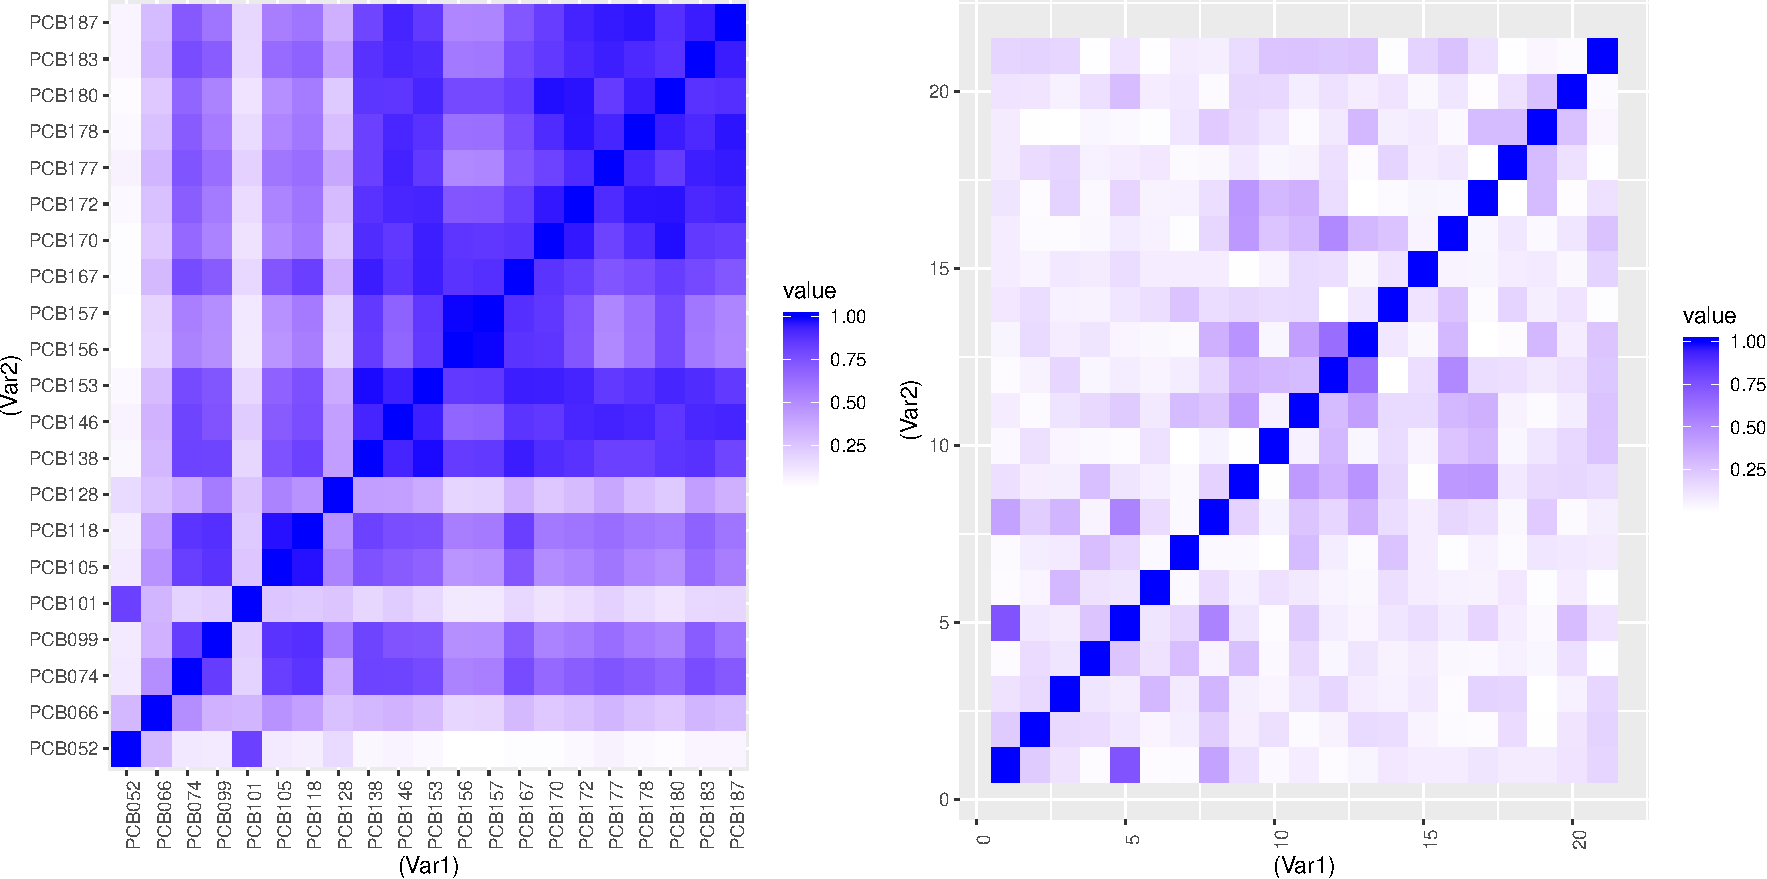
\includegraphics{PCBs_covariance_files/figure-latex/unnamed-chunk-9-1.pdf}
\caption{2003-2004}
\end{figure}

\begin{figure}
\centering
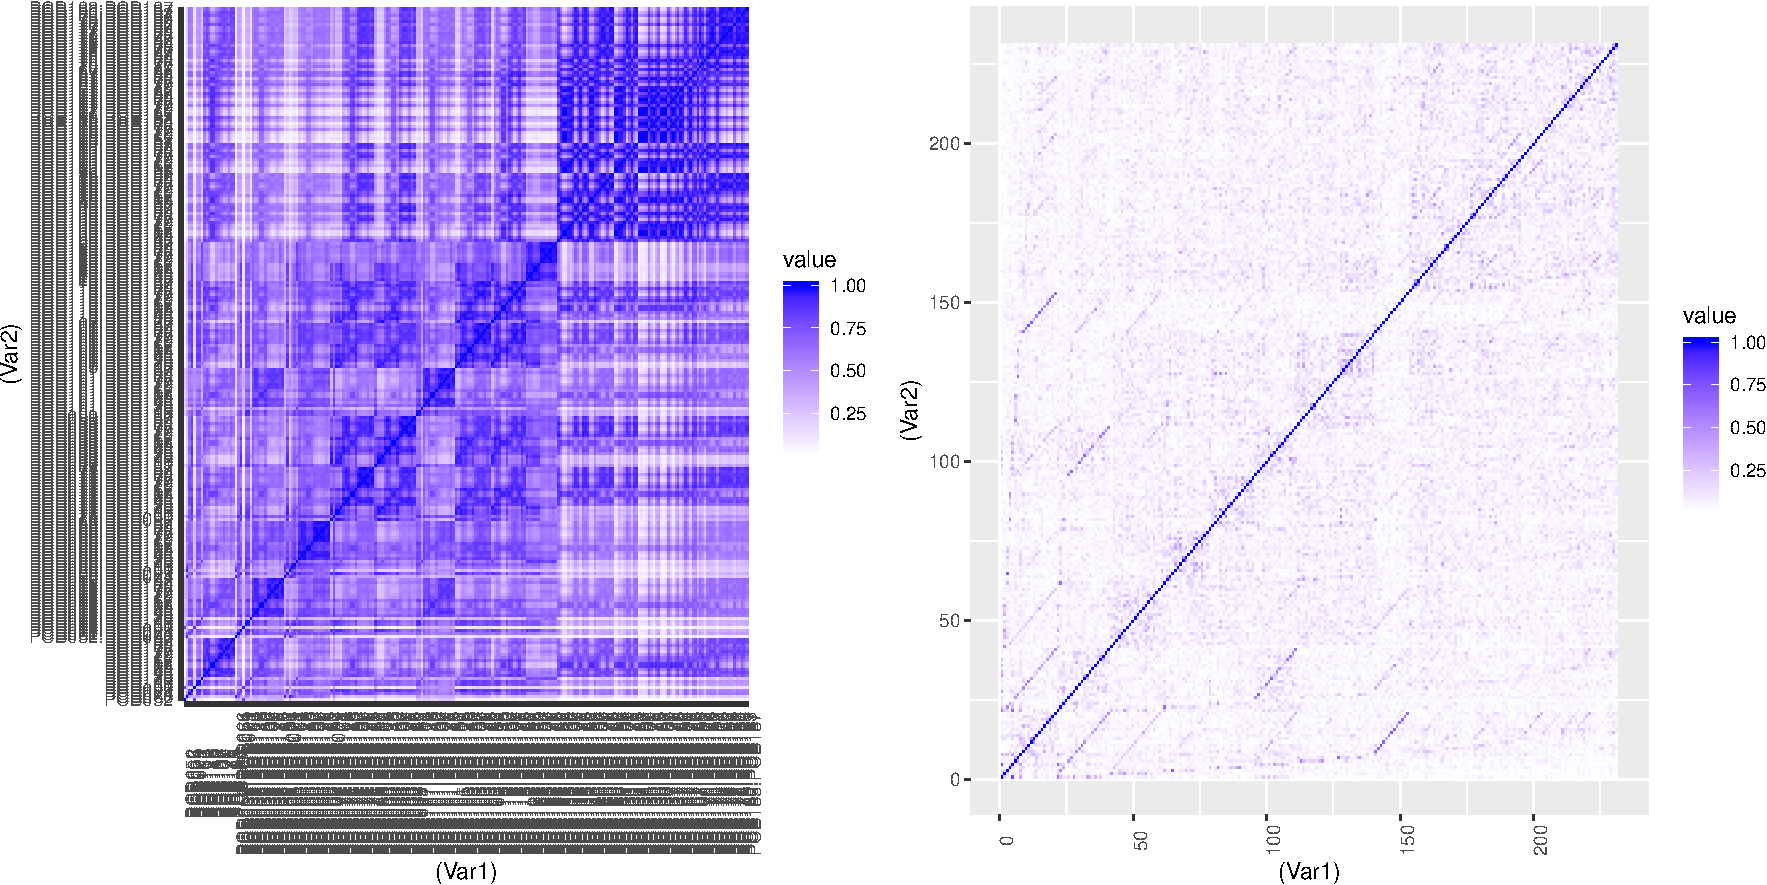
\includegraphics{PCBs_covariance_files/figure-latex/unnamed-chunk-10-1.pdf}
\caption{Combined main and interaction 1993-2004}
\end{figure}

\subsubsection{gender}\label{gender}

Followings are the heat-maps of correlation-matrix for different gender

\begin{figure}
\centering
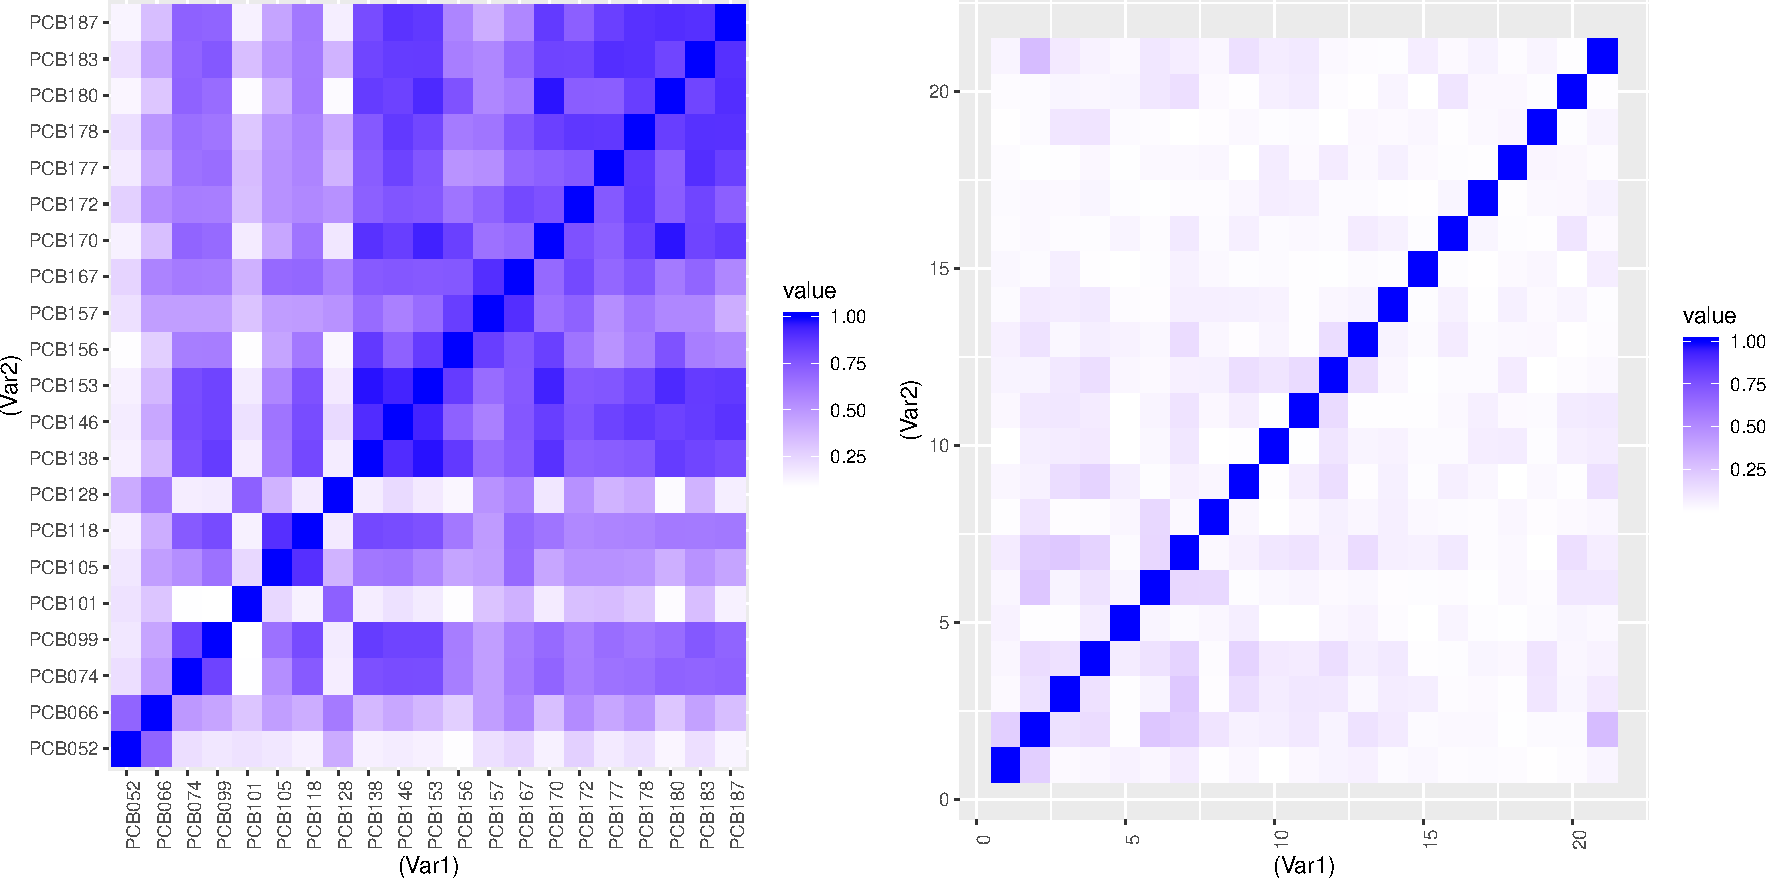
\includegraphics{PCBs_covariance_files/figure-latex/unnamed-chunk-11-1.pdf}
\caption{Male}
\end{figure}

\begin{figure}
\centering
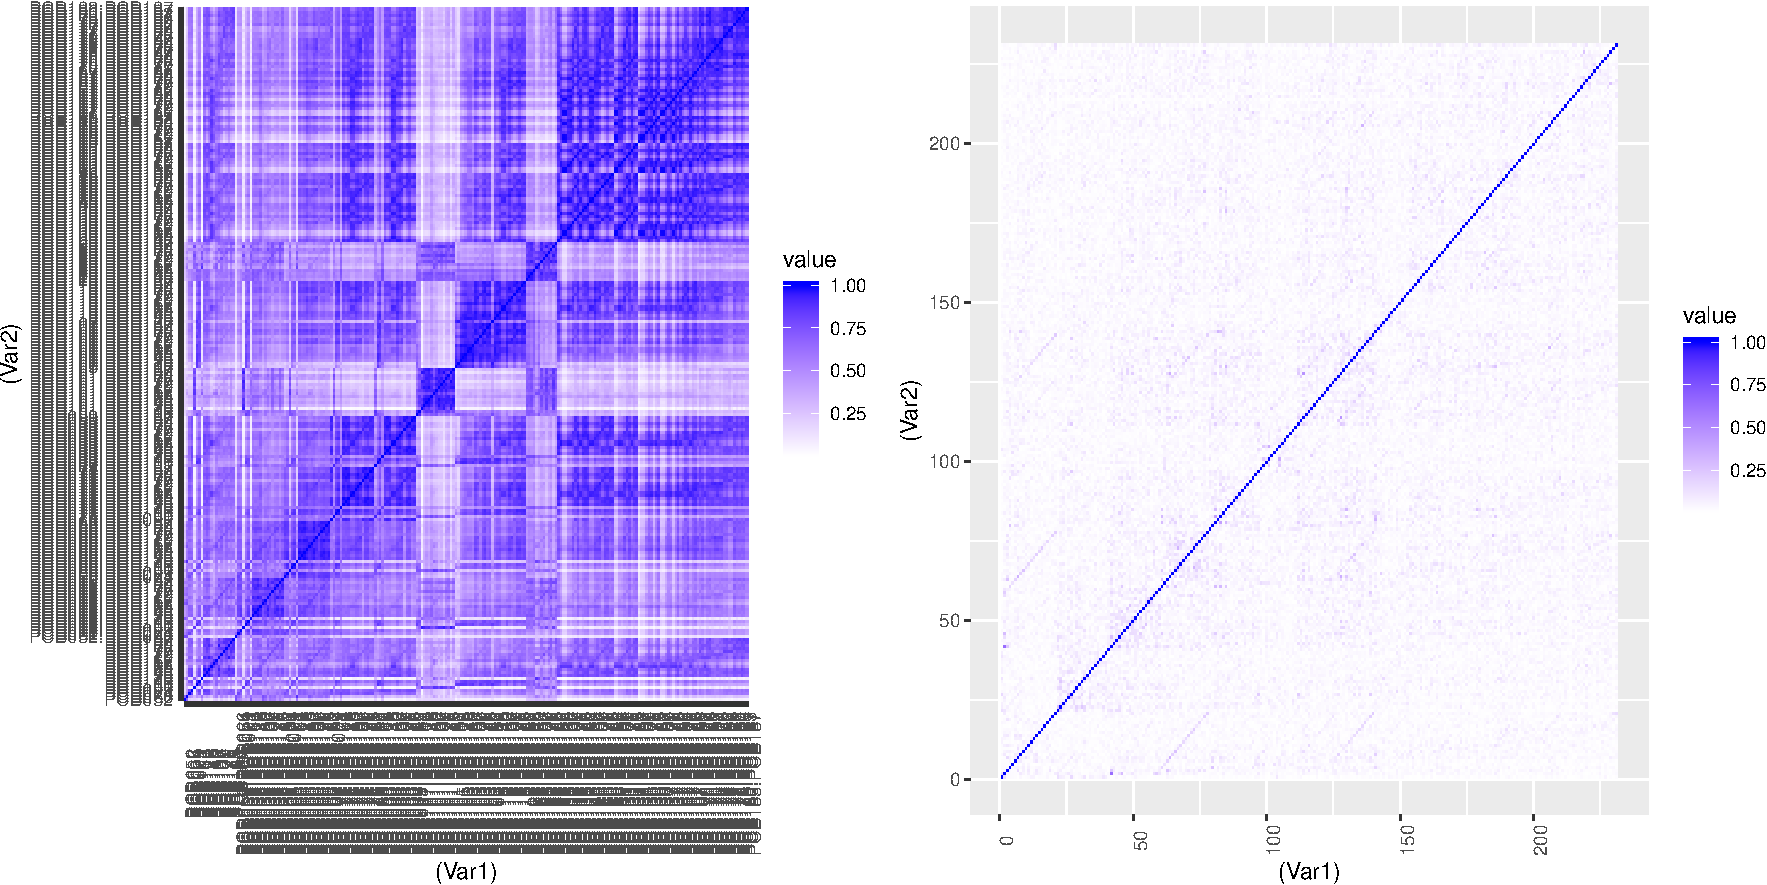
\includegraphics{PCBs_covariance_files/figure-latex/unnamed-chunk-12-1.pdf}
\caption{Combined main and interaction Male}
\end{figure}

\begin{figure}
\centering
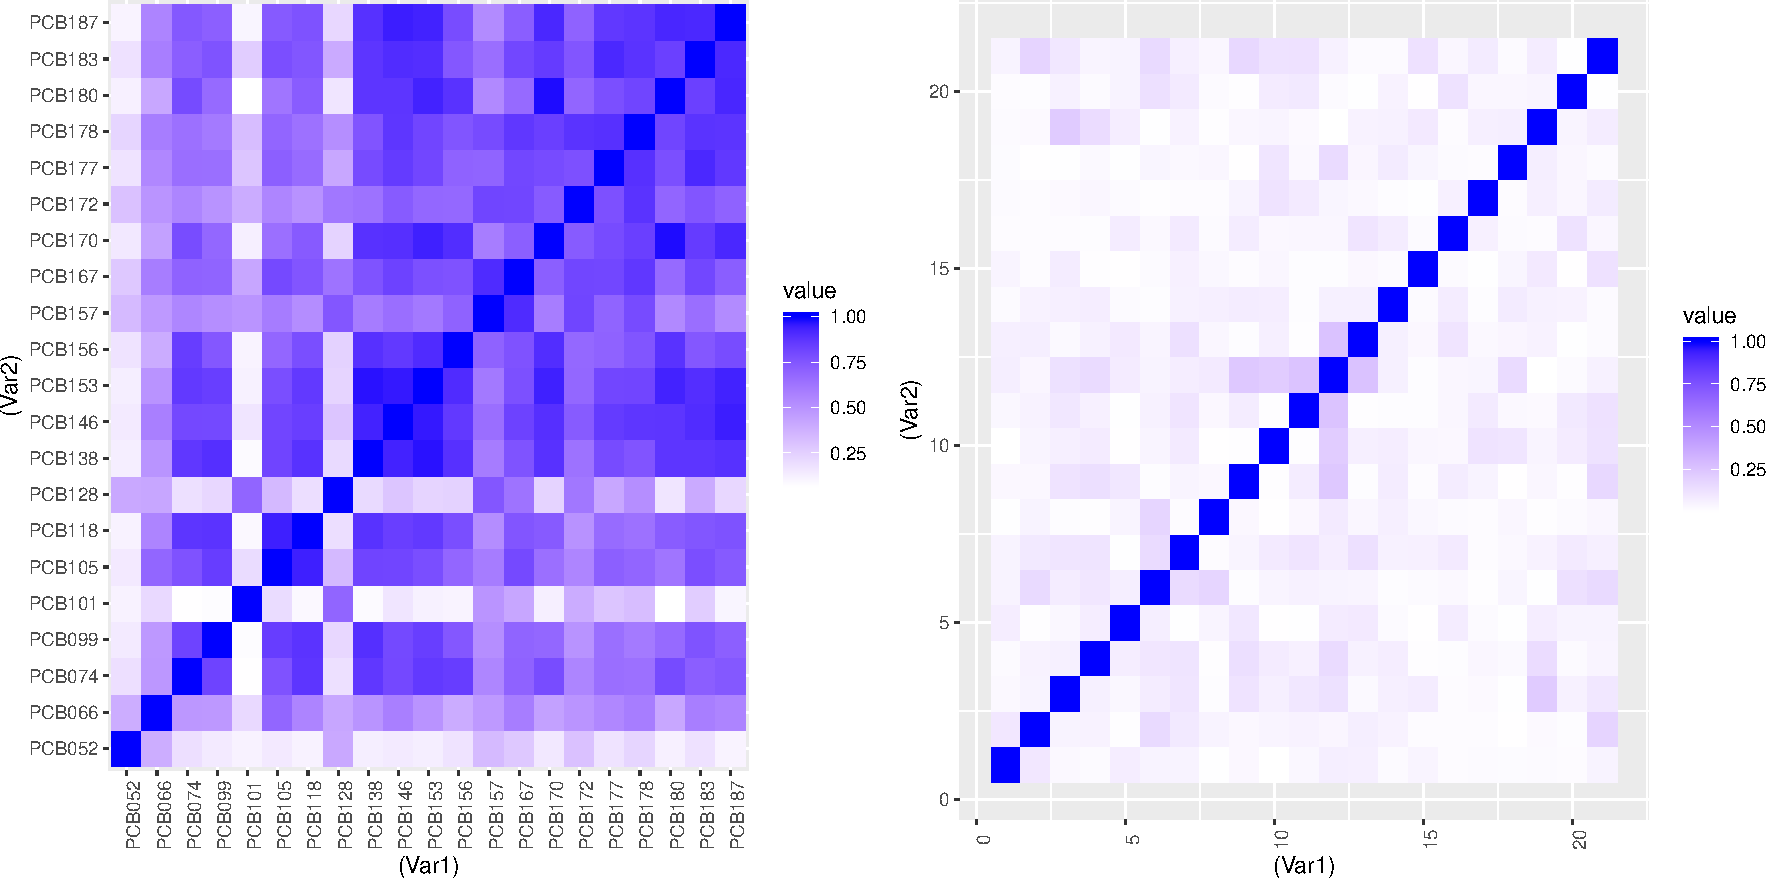
\includegraphics{PCBs_covariance_files/figure-latex/unnamed-chunk-13-1.pdf}
\caption{Female}
\end{figure}

\begin{figure}
\centering
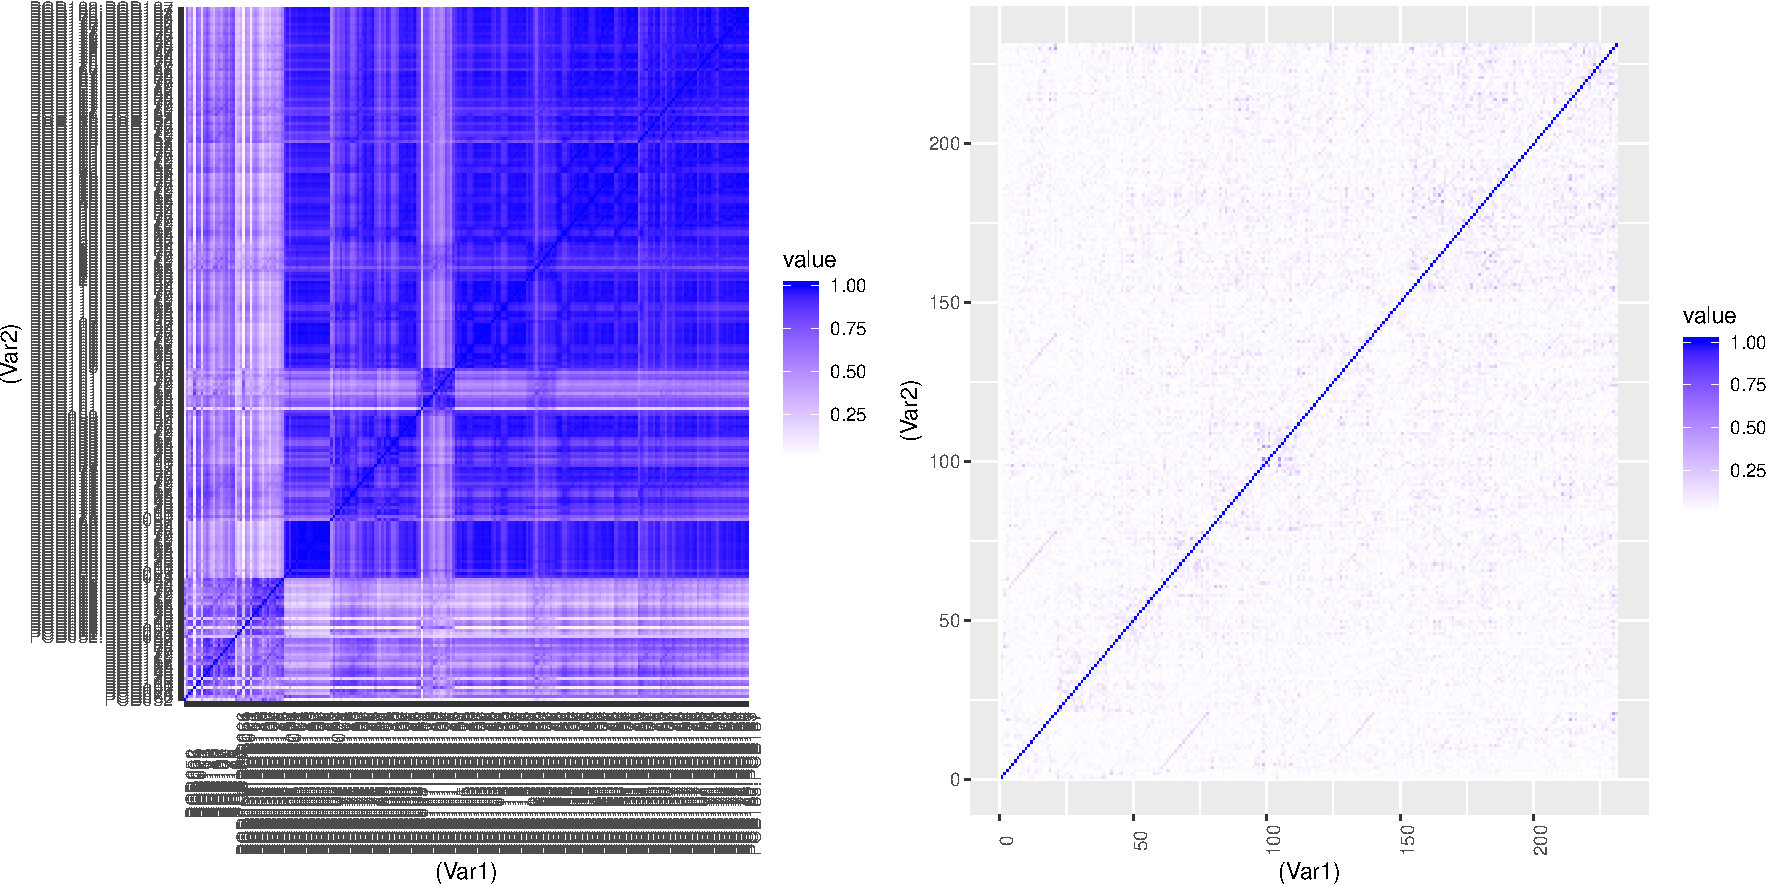
\includegraphics{PCBs_covariance_files/figure-latex/unnamed-chunk-14-1.pdf}
\caption{Combined main and interaction Female}
\end{figure}

\subsection{2005-2014}\label{section-1}

\subsubsection{the pooled-sample}\label{the-pooled-sample}

NHANES adapted a pooled sampling method to collect the PCBs data since
2005. It seems that they collect all the blood samples from all the
subjects but they only chose a sub-sample of them to measure the PCBs
value. The basic idea is following:

\begin{enumerate}
\def\labelenumi{\arabic{enumi}.}
\tightlist
\item
  Divide the whole subjects into 32 demographic groups\\
\item
  For all the subjects in each demographic group, split them into pools
  with sample size around 8. Note that the number of pools are
  proportion to the total number of subjects in the demographic group.\\
\item
  Draw a random sample from each pools, so that those sub-samples keeps
  same pattern in term of demographic groups ratio.
\end{enumerate}

The follwoing is a summary table of sub-samples of 2005-2006 subjects'
for getting PCBs measurements.
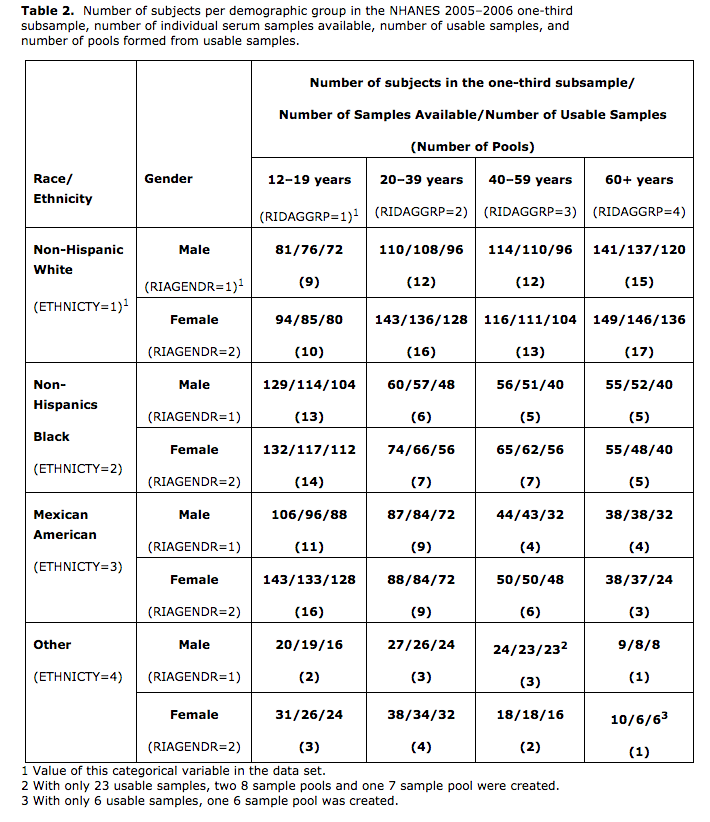
\includegraphics{./figs/subsampling_2005.png}

The types of PCBs measured for each survey is

\begin{verbatim}
$`2005`
 [1] "PCB028" "PCB044" "PCB049" "PCB052" "PCB066" "PCB074" "PCB087"
 [8] "PCB099" "PCB101" "PCB105" "PCB110" "PCB114" "PCB118" "PCB123"
[15] "PCB128" "PCB138" "PCB146" "PCB149" "PCB151" "PCB153" "PCB156"
[22] "PCB157" "PCB167" "PCB170" "PCB172" "PCB177" "PCB178" "PCB180"
[29] "PCB183" "PCB187" "PCB189" "PCB194" "PCB195" "PCB196" "PCB199"
[36] "PCB206" "PCB209"

$`2007`
 [1] "PCB028" "PCB044" "PCB049" "PCB052" "PCB066" "PCB074" "PCB087"
 [8] "PCB099" "PCB101" "PCB105" "PCB110" "PCB114" "PCB118" "PCB123"
[15] "PCB128" "PCB138" "PCB146" "PCB149" "PCB151" "PCB153" "PCB156"
[22] "PCB157" "PCB167" "PCB170" "PCB172" "PCB177" "PCB178" "PCB180"
[29] "PCB183" "PCB187" "PCB189" "PCB194" "PCB195" "PCB196" "PCB199"
[36] "PCB206" "PCB209"

$`2009`
 [1] "PCB028" "PCB066" "PCB074" "PCB099" "PCB105" "PCB114" "PCB118"
 [8] "PCB138" "PCB146" "PCB153" "PCB156" "PCB157" "PCB167" "PCB170"
[15] "PCB178" "PCB180" "PCB183" "PCB187" "PCB189" "PCB194" "PCB196"
[22] "PCB199" "PCB206" "PCB209"

$`2011`
 [1] "PCB028" "PCB066" "PCB074" "PCB099" "PCB105" "PCB114" "PCB118"
 [8] "PCB138" "PCB146" "PCB153" "PCB156" "PCB157" "PCB167" "PCB170"
[15] "PCB178" "PCB180" "PCB183" "PCB187" "PCB189" "PCB194" "PCB196"
[22] "PCB199" "PCB206" "PCB209"

$`2013`
 [1] "PCB028" "PCB066" "PCB074" "PCB099" "PCB105" "PCB114" "PCB118"
 [8] "PCB138" "PCB146" "PCB153" "PCB156" "PCB157" "PCB167" "PCB170"
[15] "PCB178" "PCB180" "PCB183" "PCB187" "PCB189" "PCB194" "PCB196"
[22] "PCB199" "PCB206" "PCB209"
\end{verbatim}

The common PCBs that were measured by each survey is

\begin{verbatim}
 [1] "PCB028" "PCB066" "PCB074" "PCB099" "PCB105" "PCB114" "PCB118"
 [8] "PCB138" "PCB146" "PCB153" "PCB156" "PCB157" "PCB167" "PCB170"
[15] "PCB178" "PCB180" "PCB183" "PCB187" "PCB189" "PCB194" "PCB196"
[22] "PCB199" "PCB206" "PCB209"
\end{verbatim}

I will use those 24 PCBs to calculate their covariance matrix.

The total number of PCBs data from 2005-2014 is 1347. After I remove all
the missing data, what I get is total 1228 observations.

Note that I only work on the PCBs measurement without adjustment, but I
used the under the limit adjustment.

\newpage

\subsubsection{time}\label{time-1}

Followings are 5 heat-maps of correlation-matrix across the 3 surveys.
In general, they have high correlations among those PCBs. But they do
show some common pattern.

The number of observation across each survey is

\begin{verbatim}
   SDDSRVYR   N
1:        4 247
2:        5 264
3:        6 215
4:        7 248
5:        8 254
\end{verbatim}

\newpage 

\begin{figure}
\centering
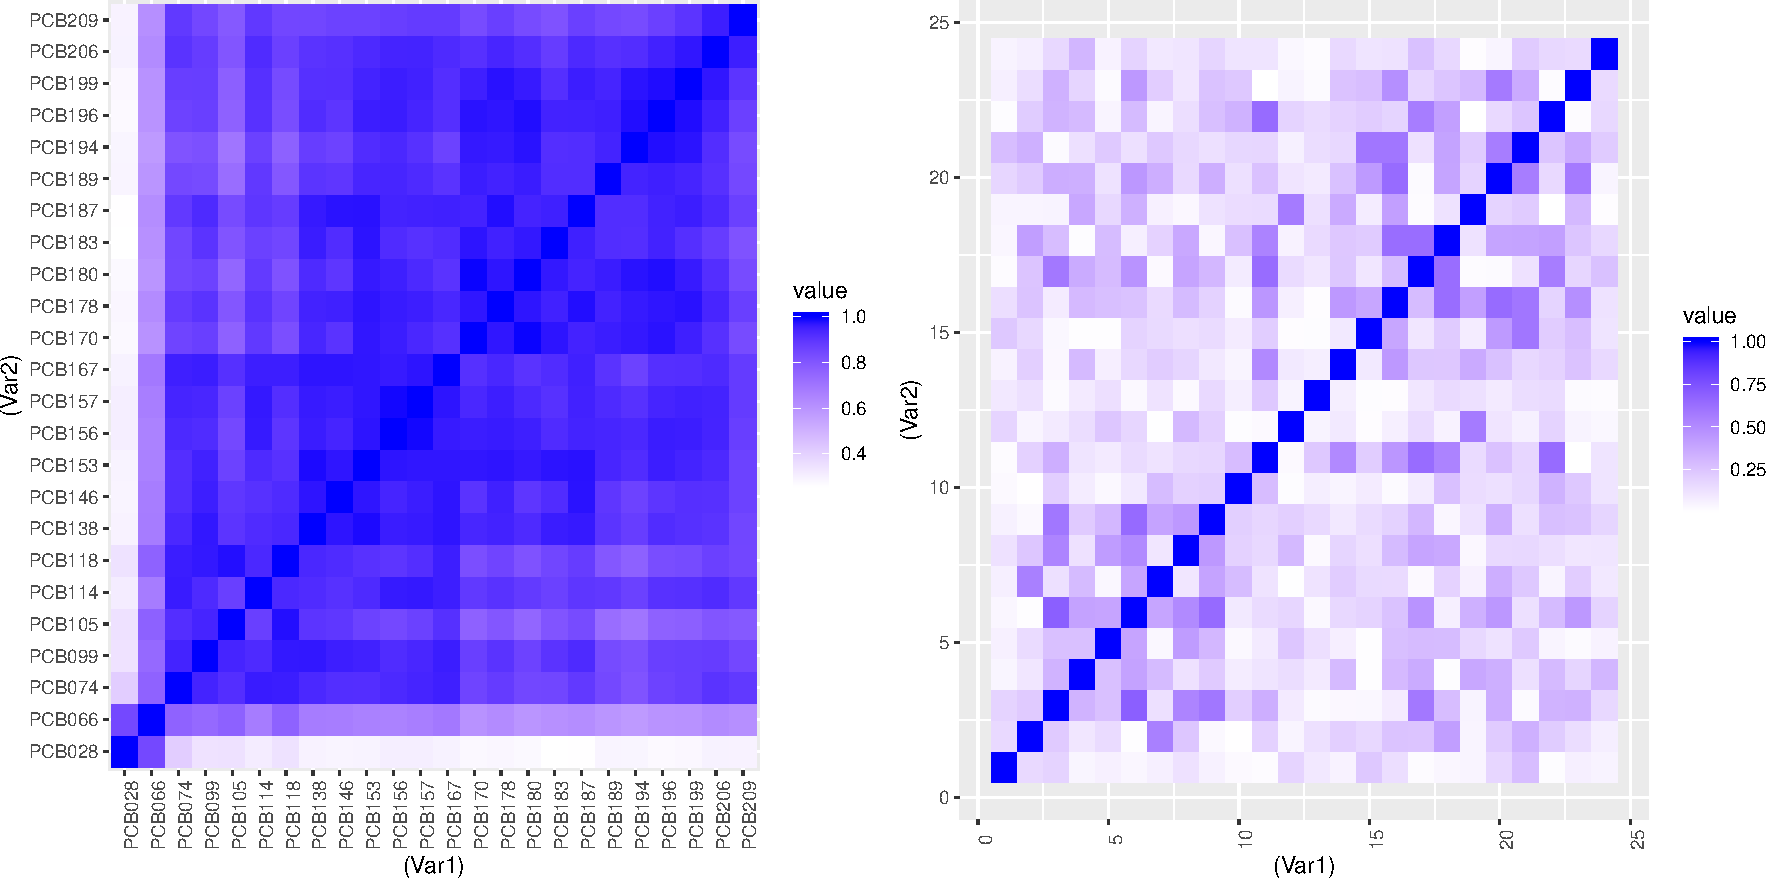
\includegraphics{PCBs_covariance_files/figure-latex/unnamed-chunk-19-1.pdf}
\caption{2005-2006}
\end{figure}

\begin{figure}
\centering
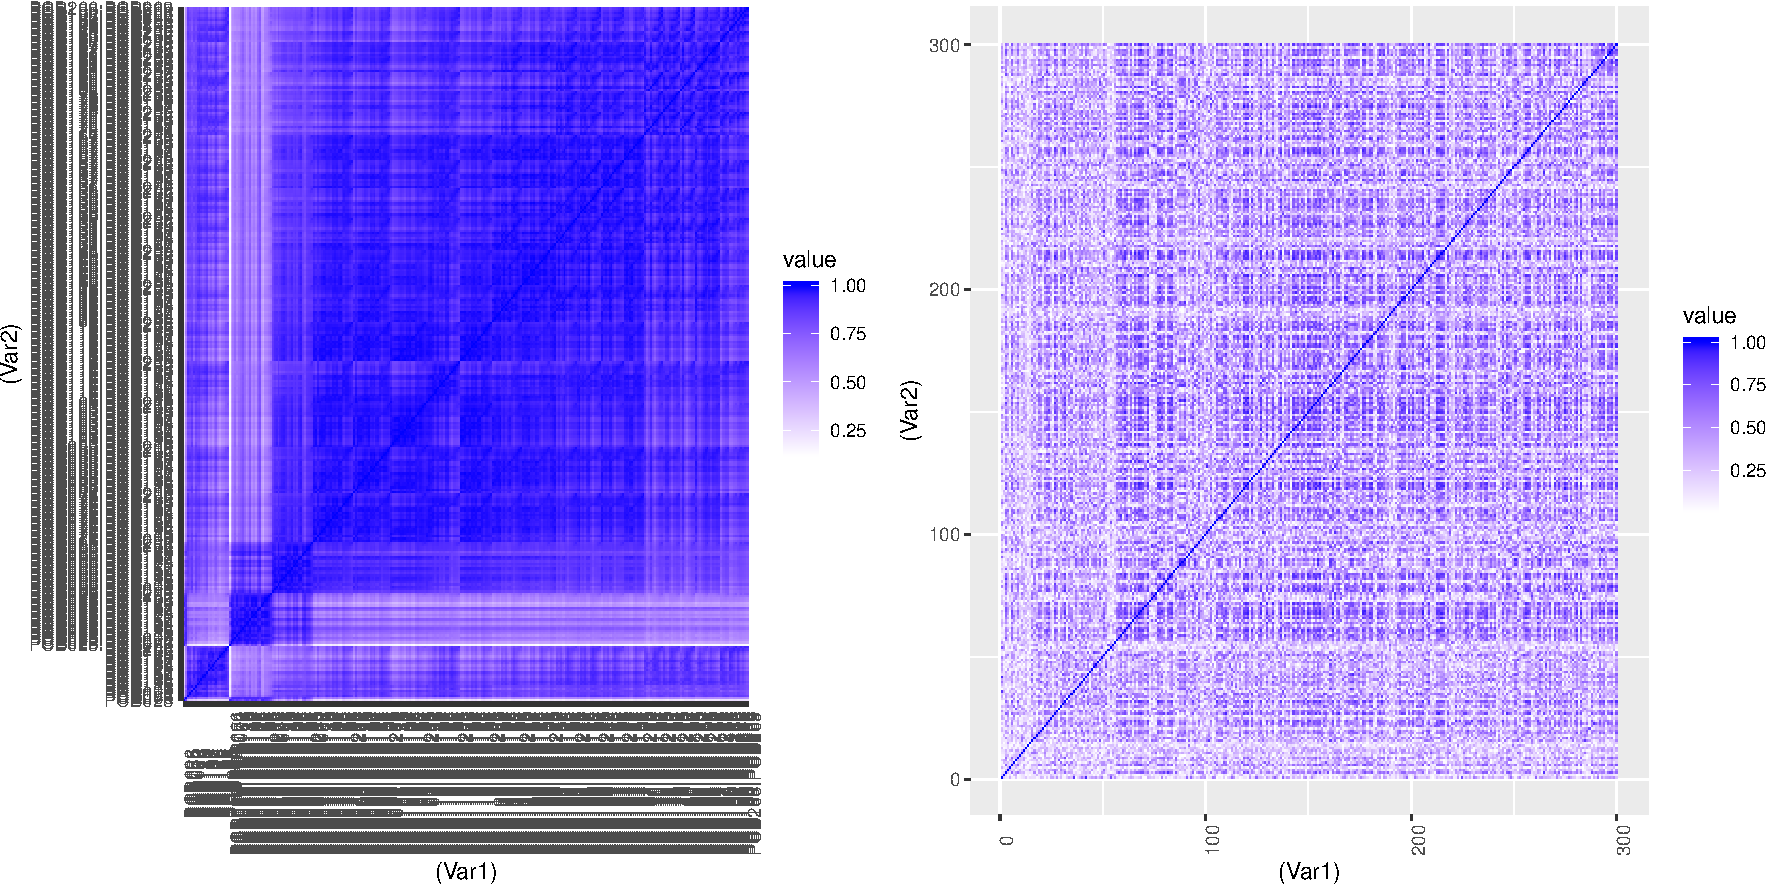
\includegraphics{PCBs_covariance_files/figure-latex/unnamed-chunk-20-1.pdf}
\caption{Combined main and interaction 2005-2006}
\end{figure}

\begin{figure}
\centering
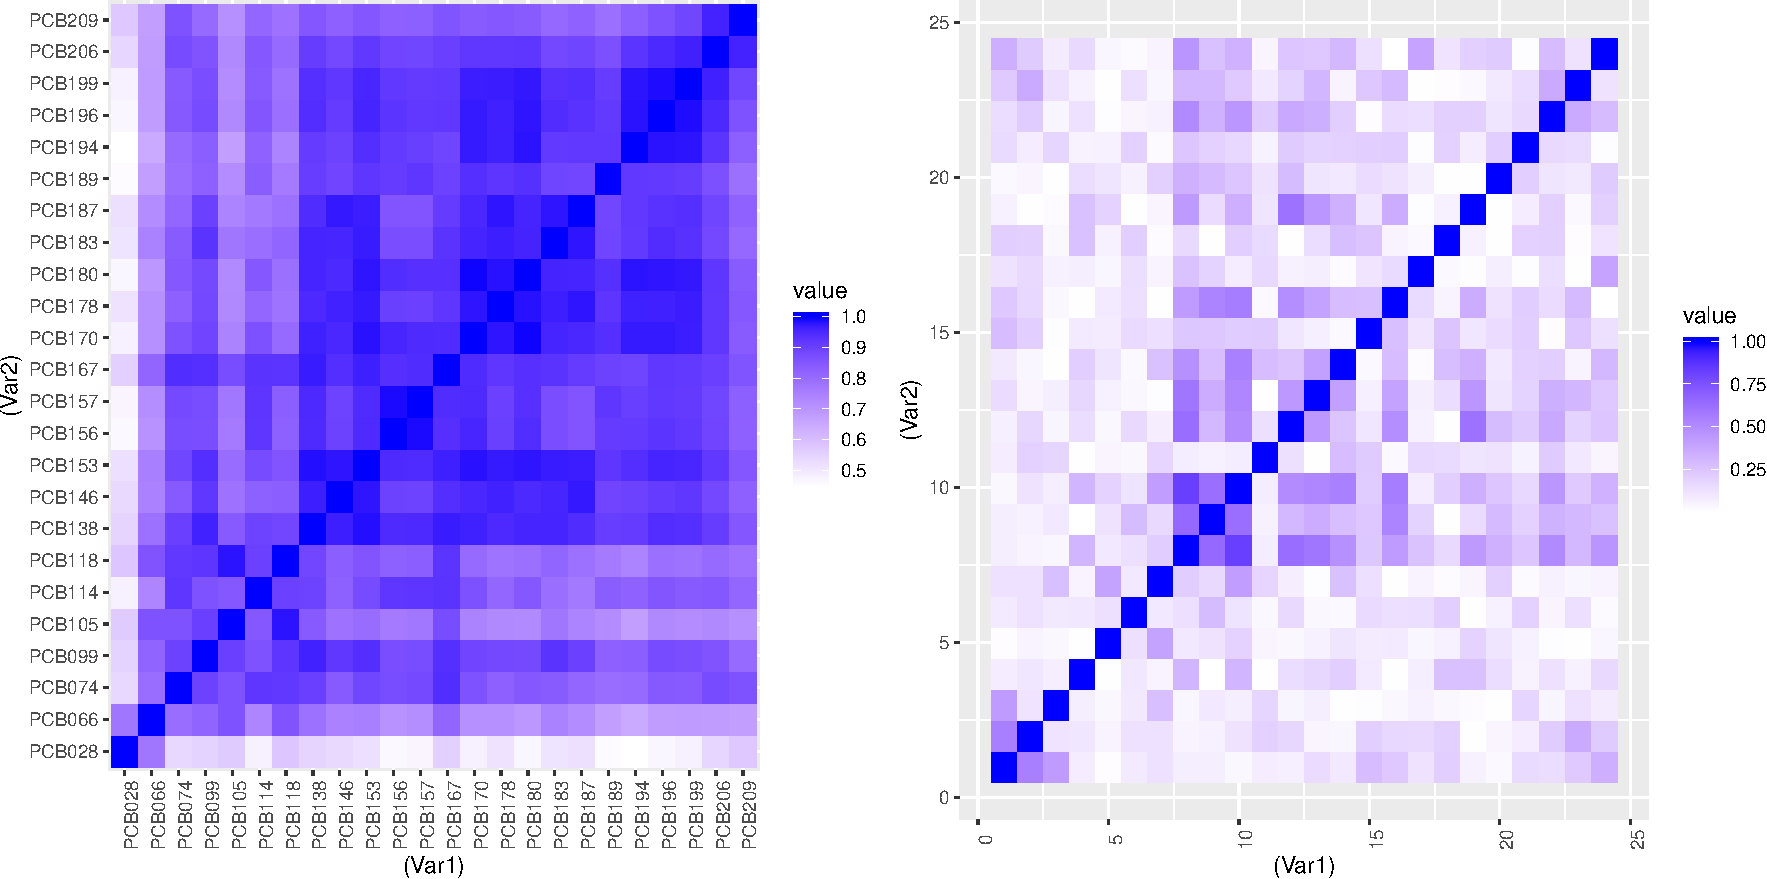
\includegraphics{PCBs_covariance_files/figure-latex/unnamed-chunk-21-1.pdf}
\caption{2007-2008}
\end{figure}

\begin{figure}
\centering
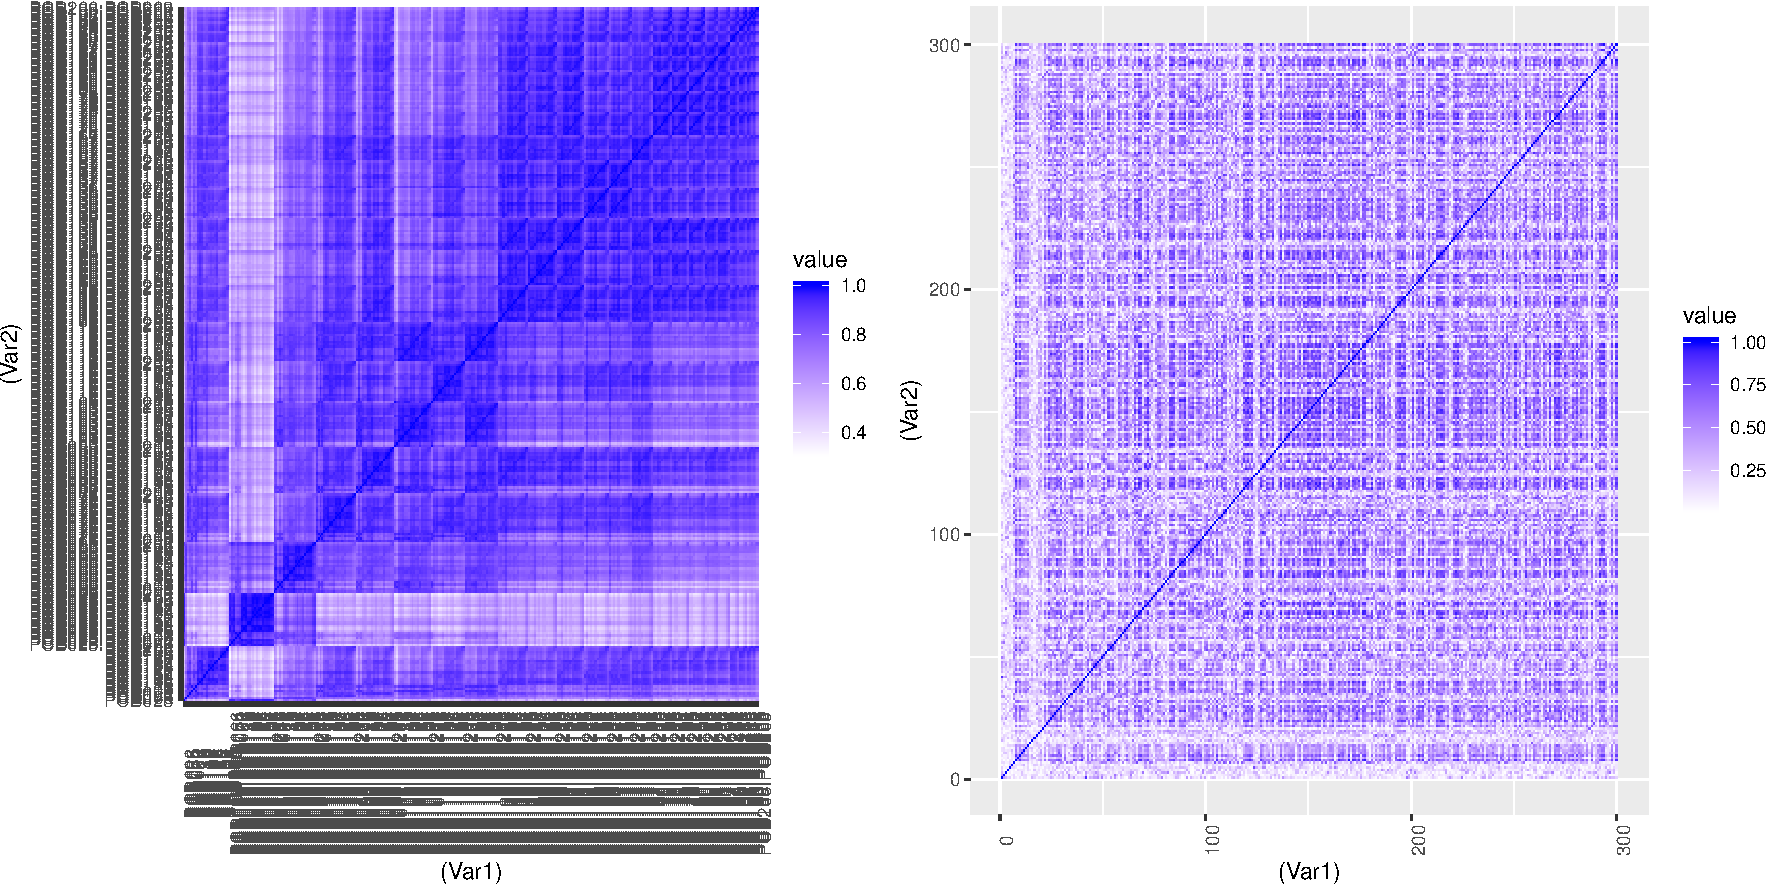
\includegraphics{PCBs_covariance_files/figure-latex/unnamed-chunk-22-1.pdf}
\caption{Combined main and interaction 2007-2008}
\end{figure}

\begin{figure}
\centering
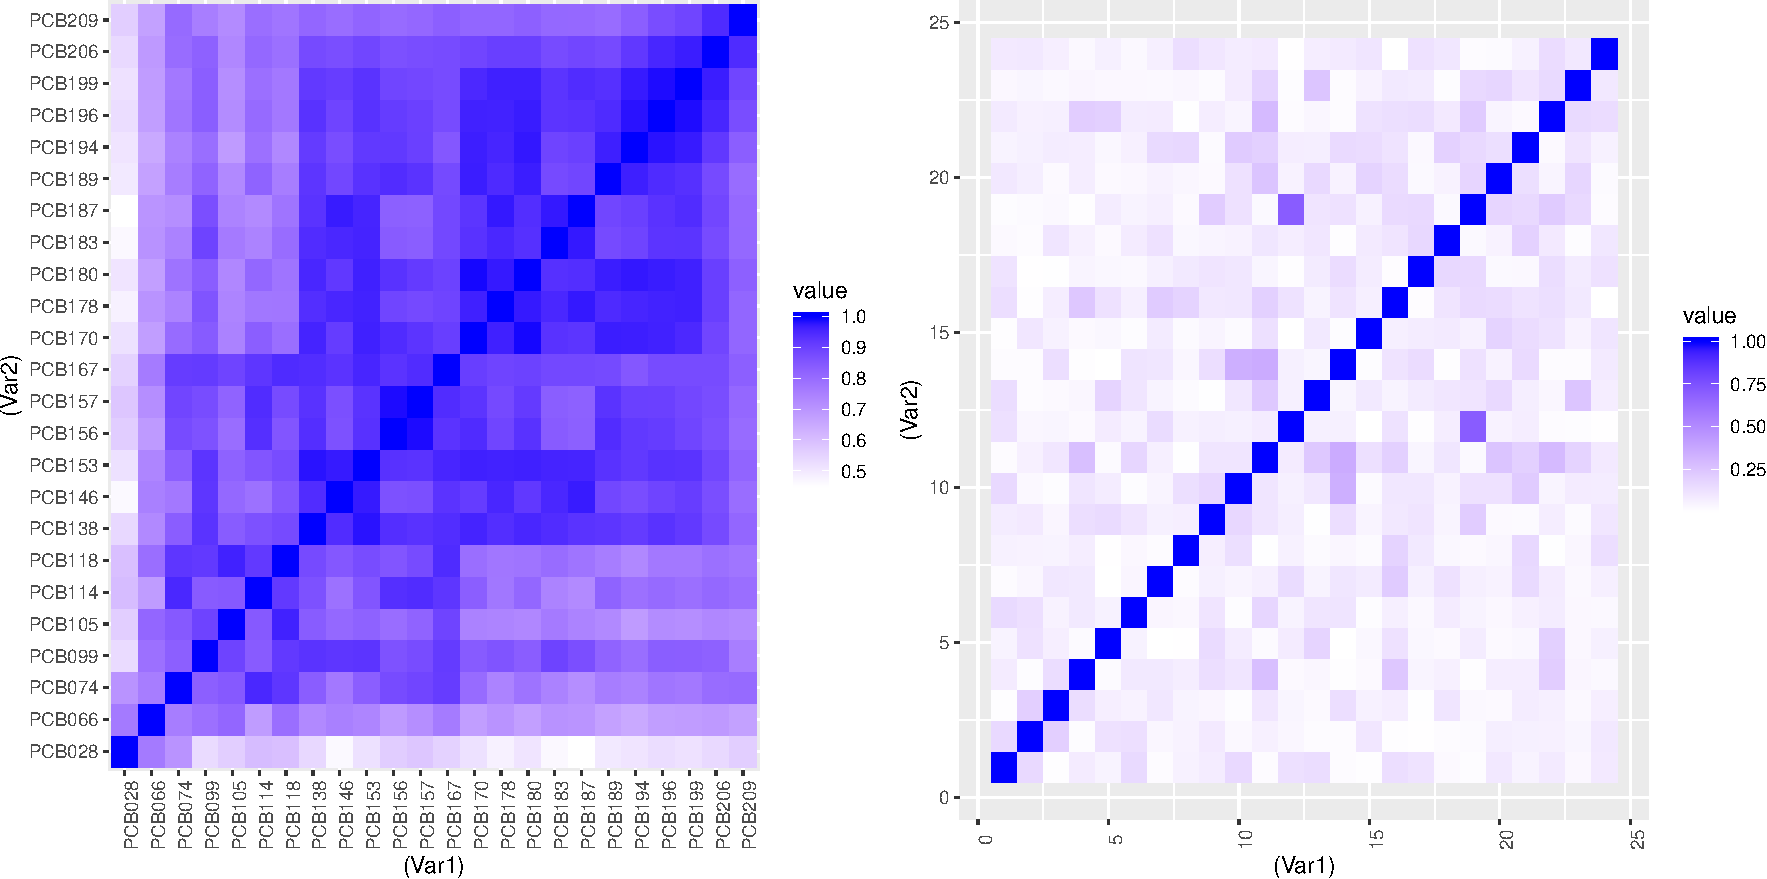
\includegraphics{PCBs_covariance_files/figure-latex/unnamed-chunk-23-1.pdf}
\caption{2009-2010}
\end{figure}

\begin{figure}
\centering
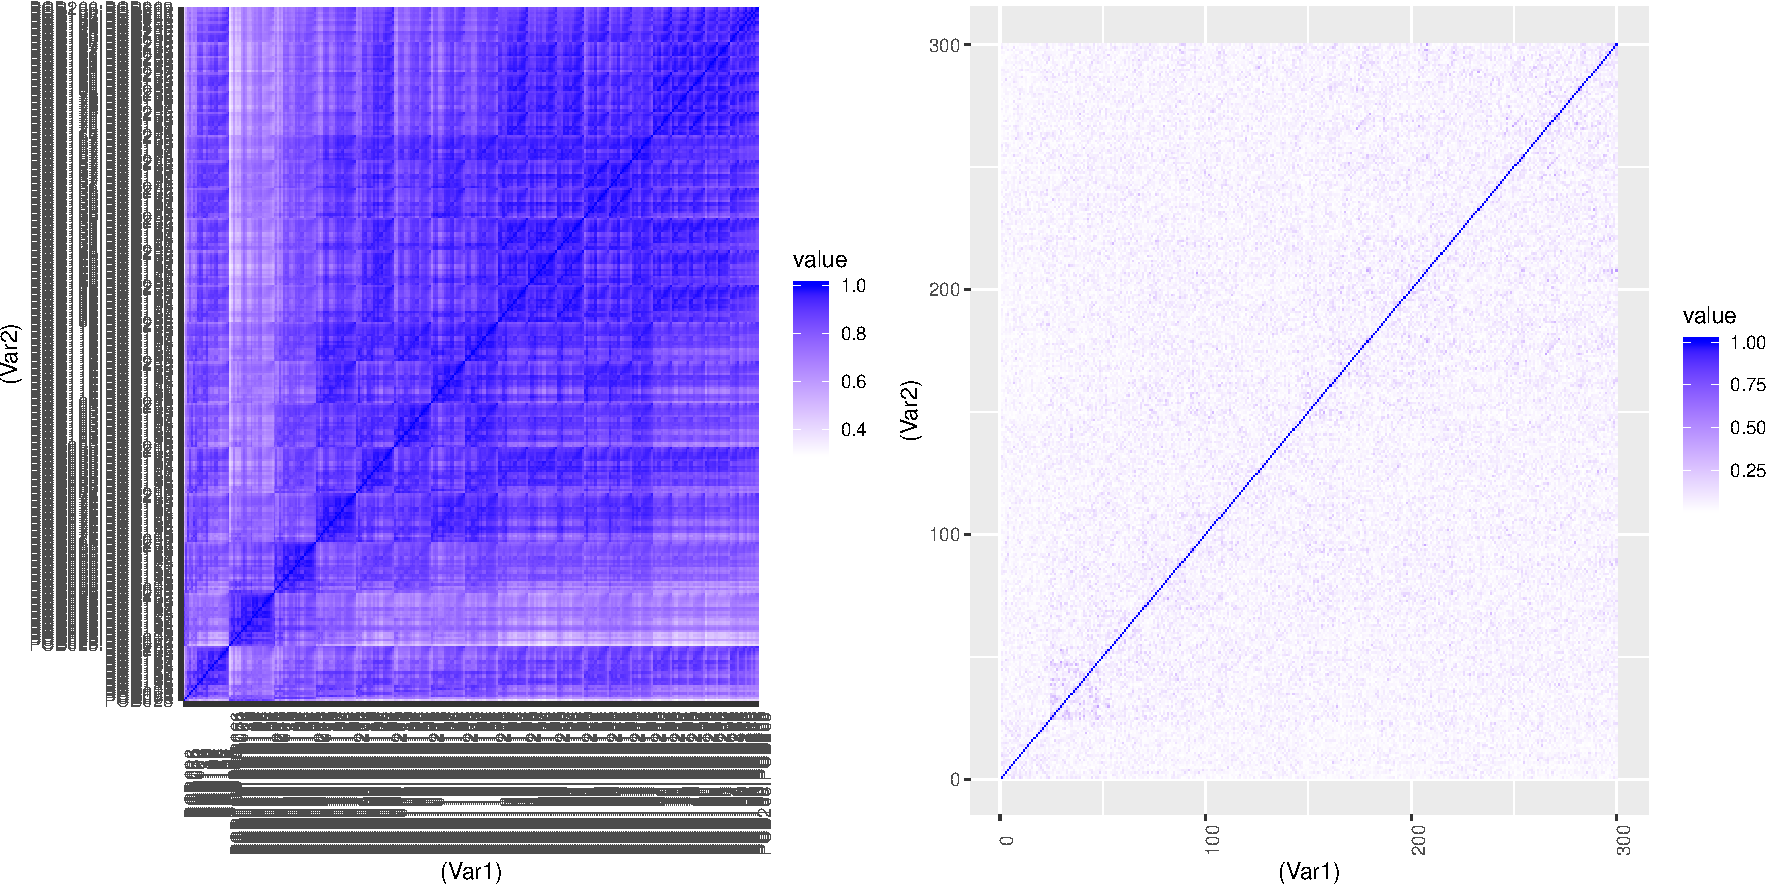
\includegraphics{PCBs_covariance_files/figure-latex/unnamed-chunk-24-1.pdf}
\caption{Combined main and interaction 2009-2010}
\end{figure}

\begin{figure}
\centering
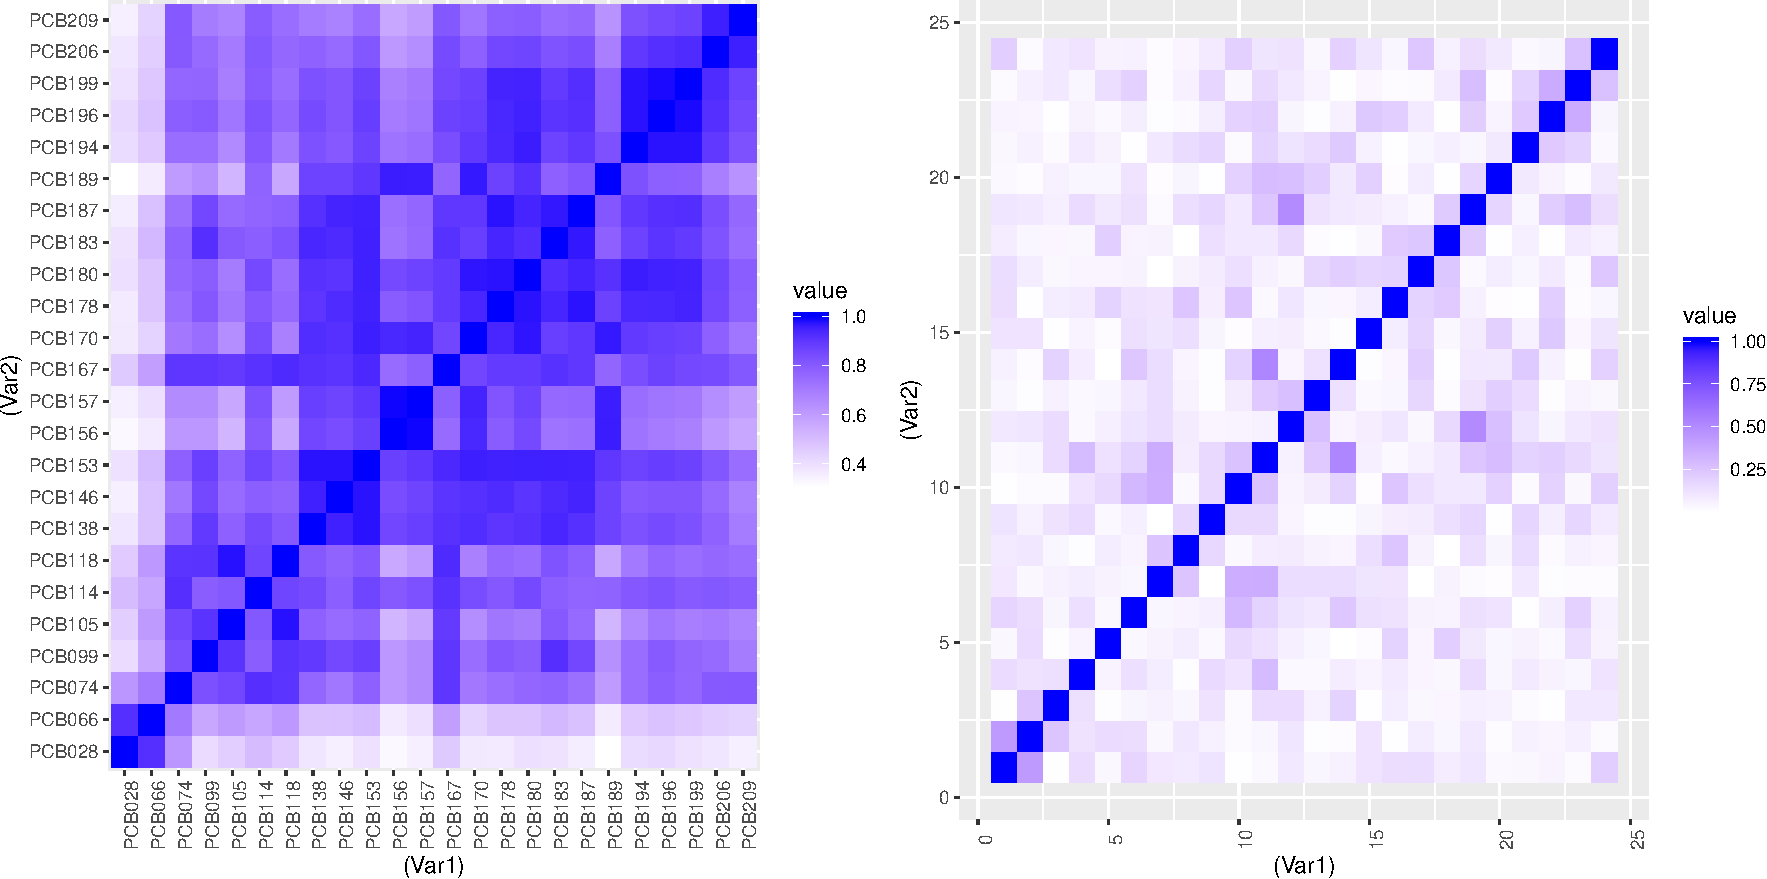
\includegraphics{PCBs_covariance_files/figure-latex/unnamed-chunk-25-1.pdf}
\caption{2011-2012}
\end{figure}

\begin{figure}
\centering
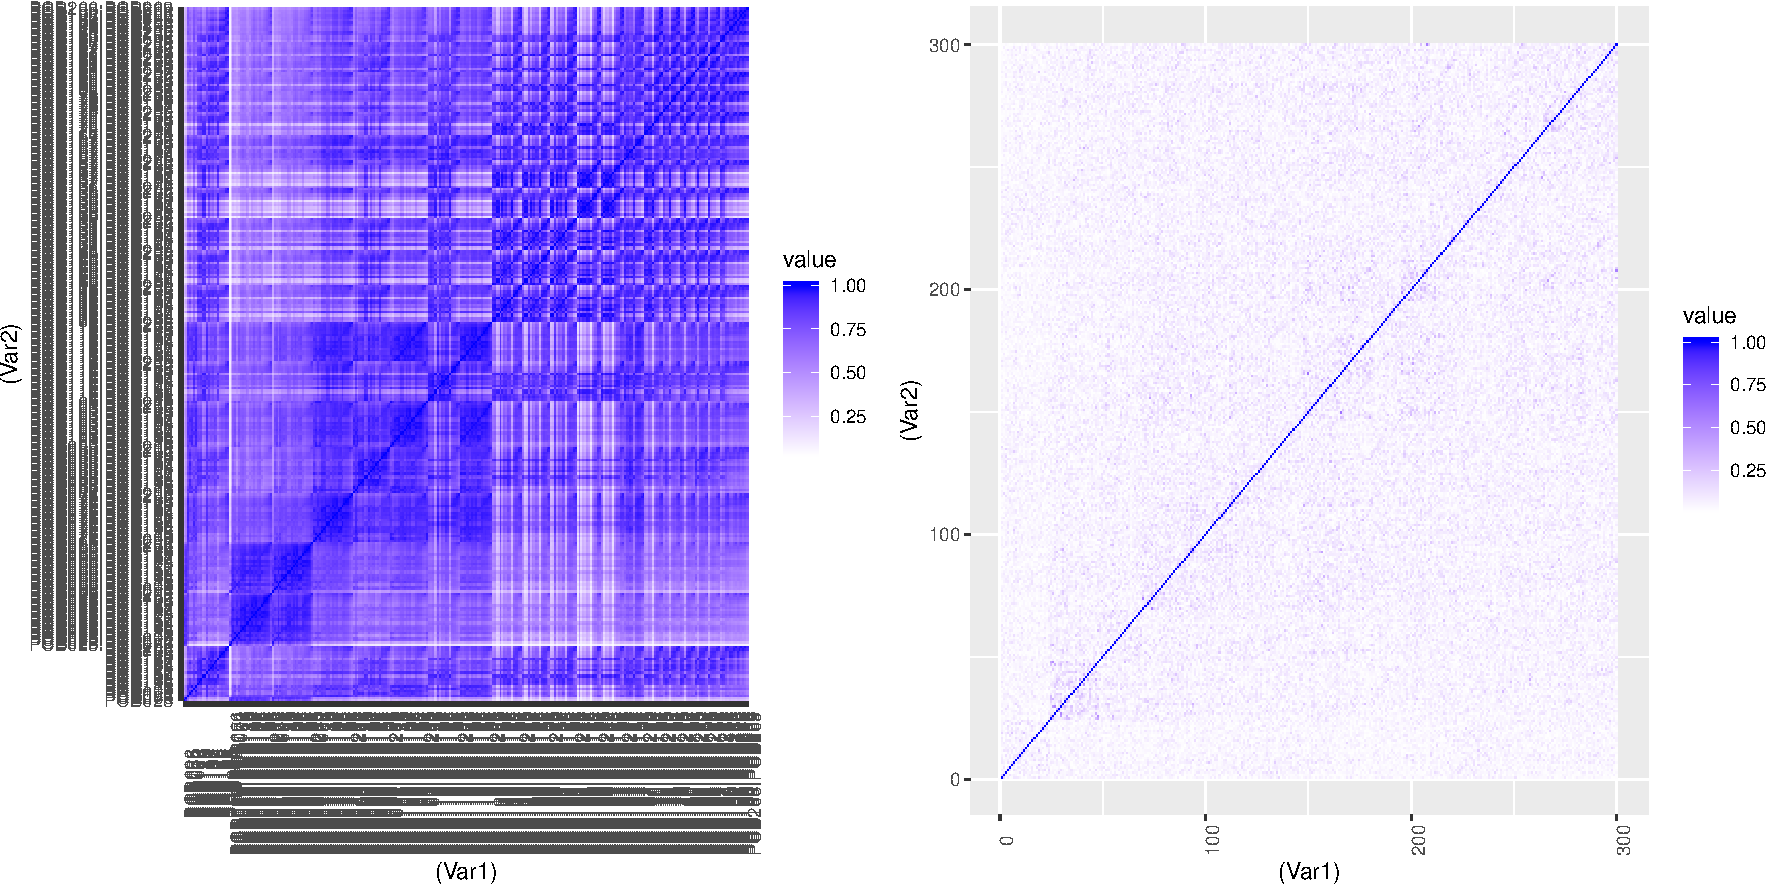
\includegraphics{PCBs_covariance_files/figure-latex/unnamed-chunk-26-1.pdf}
\caption{Combined main and interaction 2011-2012}
\end{figure}

\begin{figure}
\centering
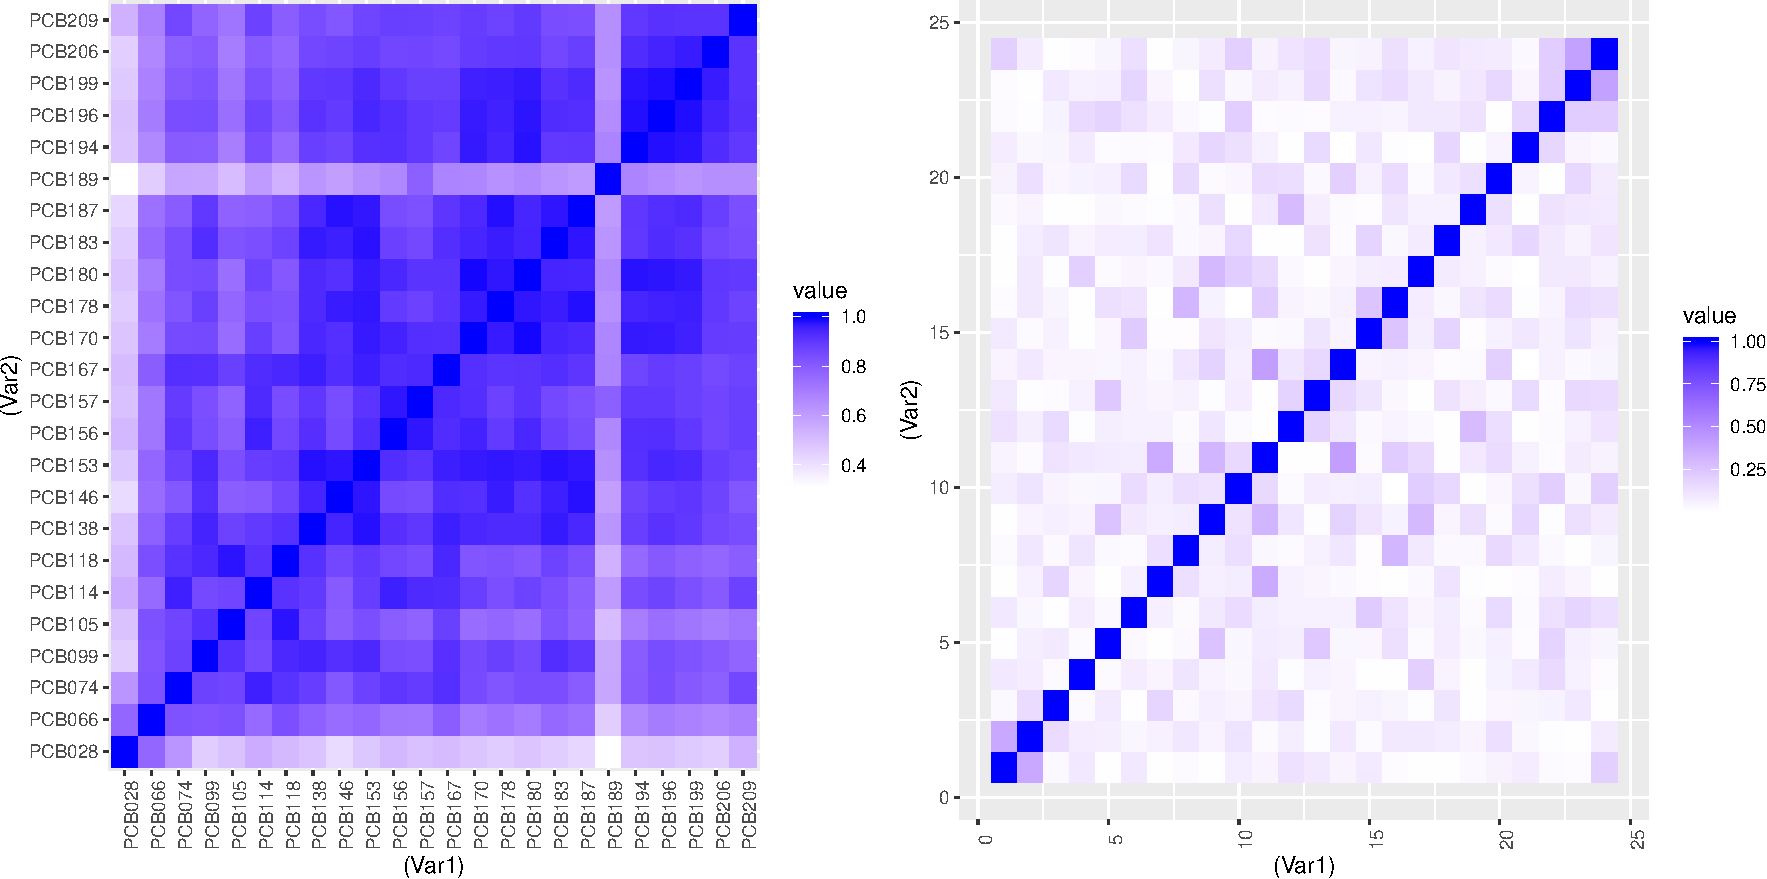
\includegraphics{PCBs_covariance_files/figure-latex/unnamed-chunk-27-1.pdf}
\caption{2013-2014}
\end{figure}

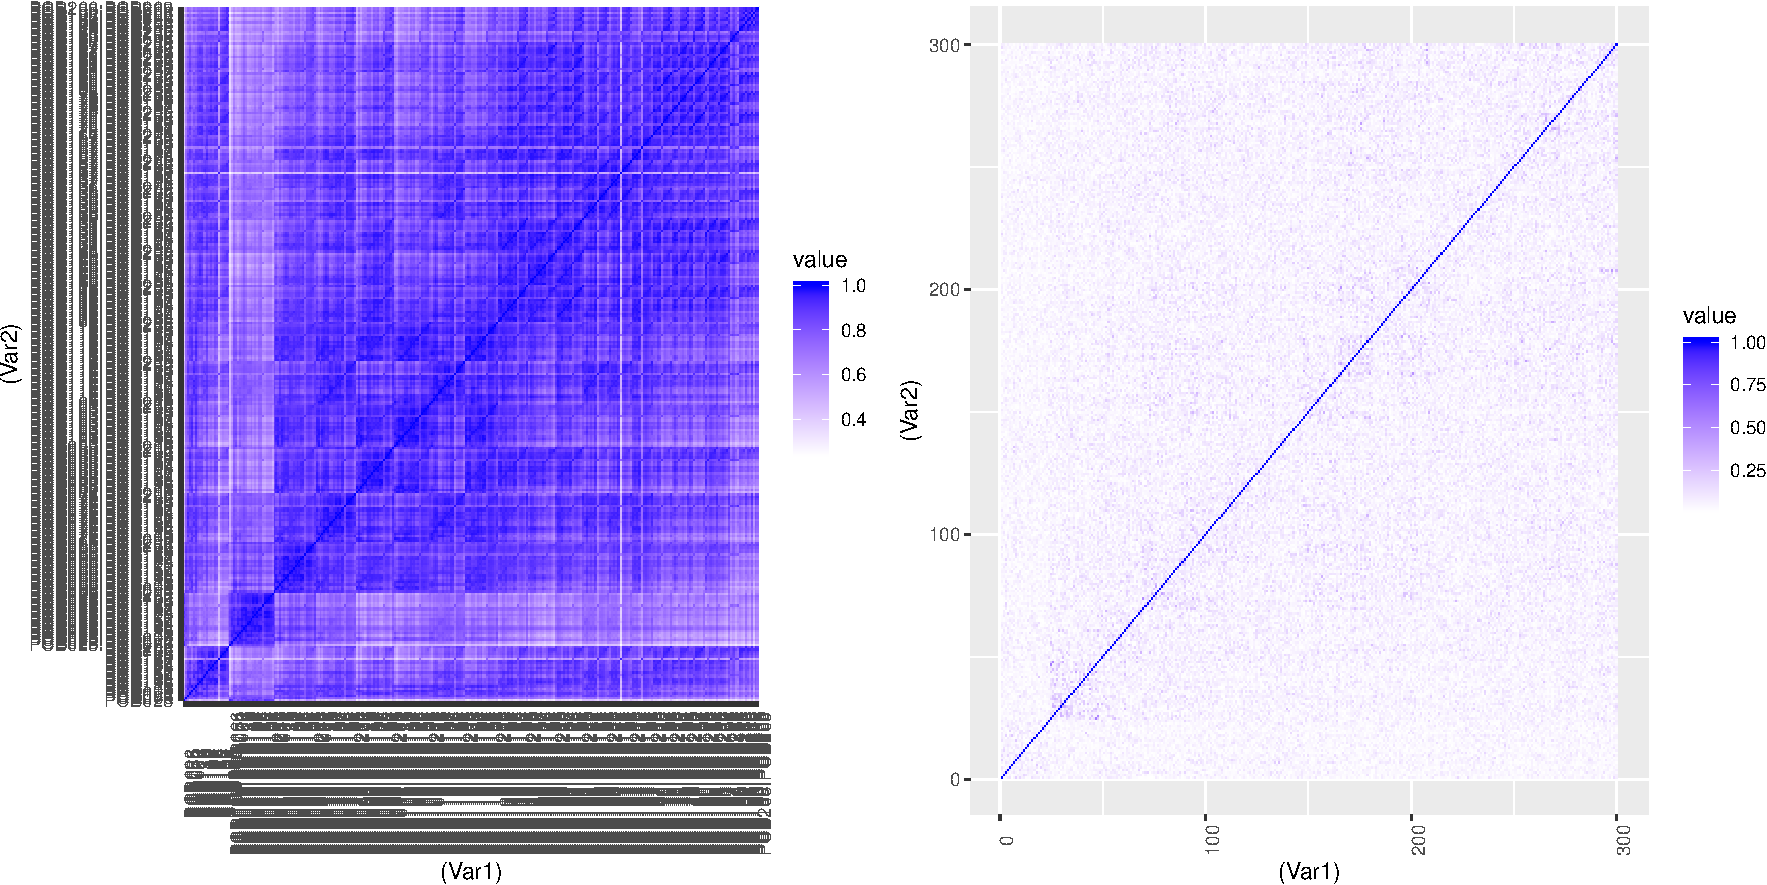
\includegraphics{PCBs_covariance_files/figure-latex/unnamed-chunk-28-1.pdf}
\#\#\# gender Followings are the heat-maps of correlation-matrix for
different gender

\begin{figure}
\centering
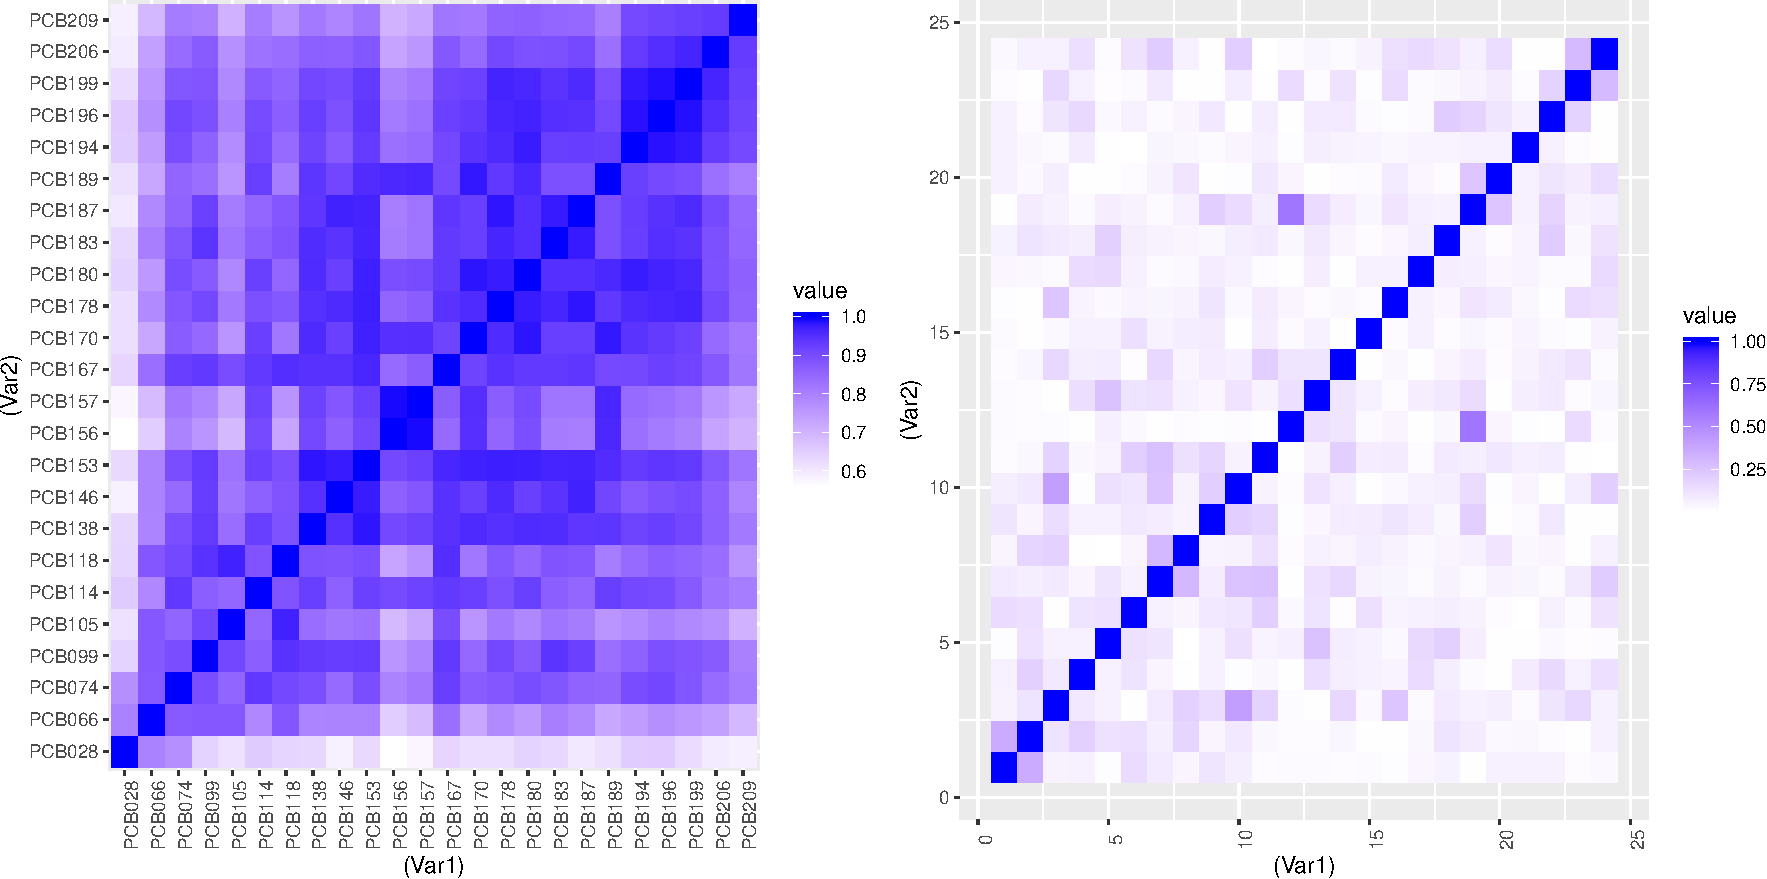
\includegraphics{PCBs_covariance_files/figure-latex/unnamed-chunk-29-1.pdf}
\caption{Male}
\end{figure}

\begin{figure}
\centering
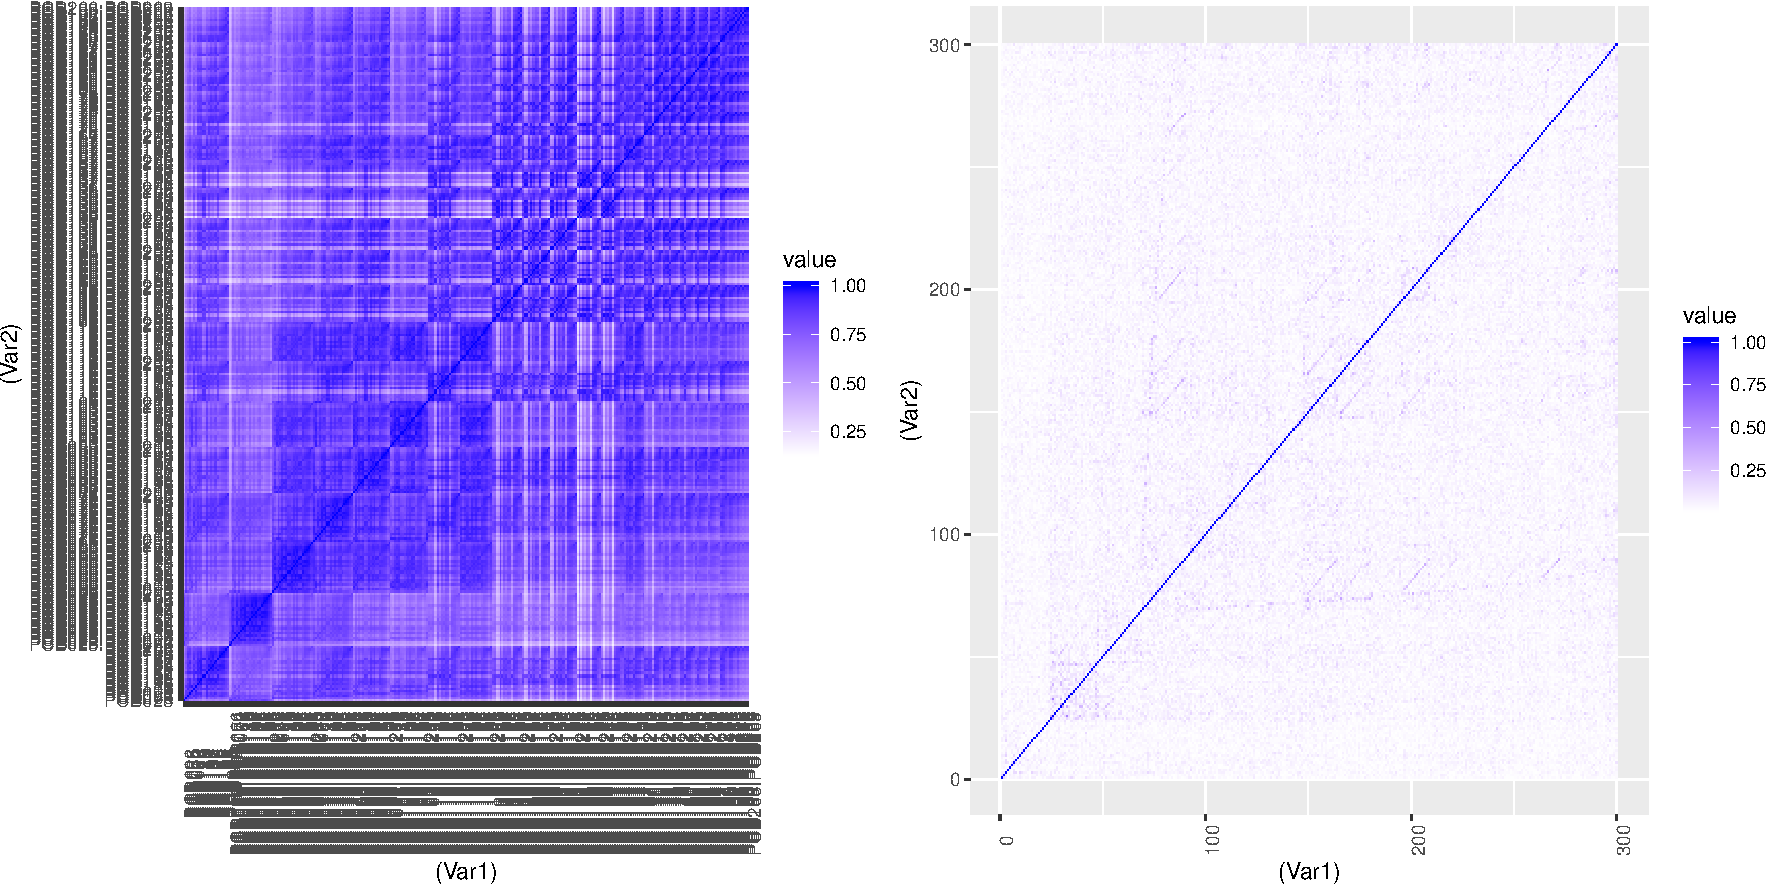
\includegraphics{PCBs_covariance_files/figure-latex/unnamed-chunk-30-1.pdf}
\caption{Combined main and interaction Male}
\end{figure}

\begin{figure}
\centering
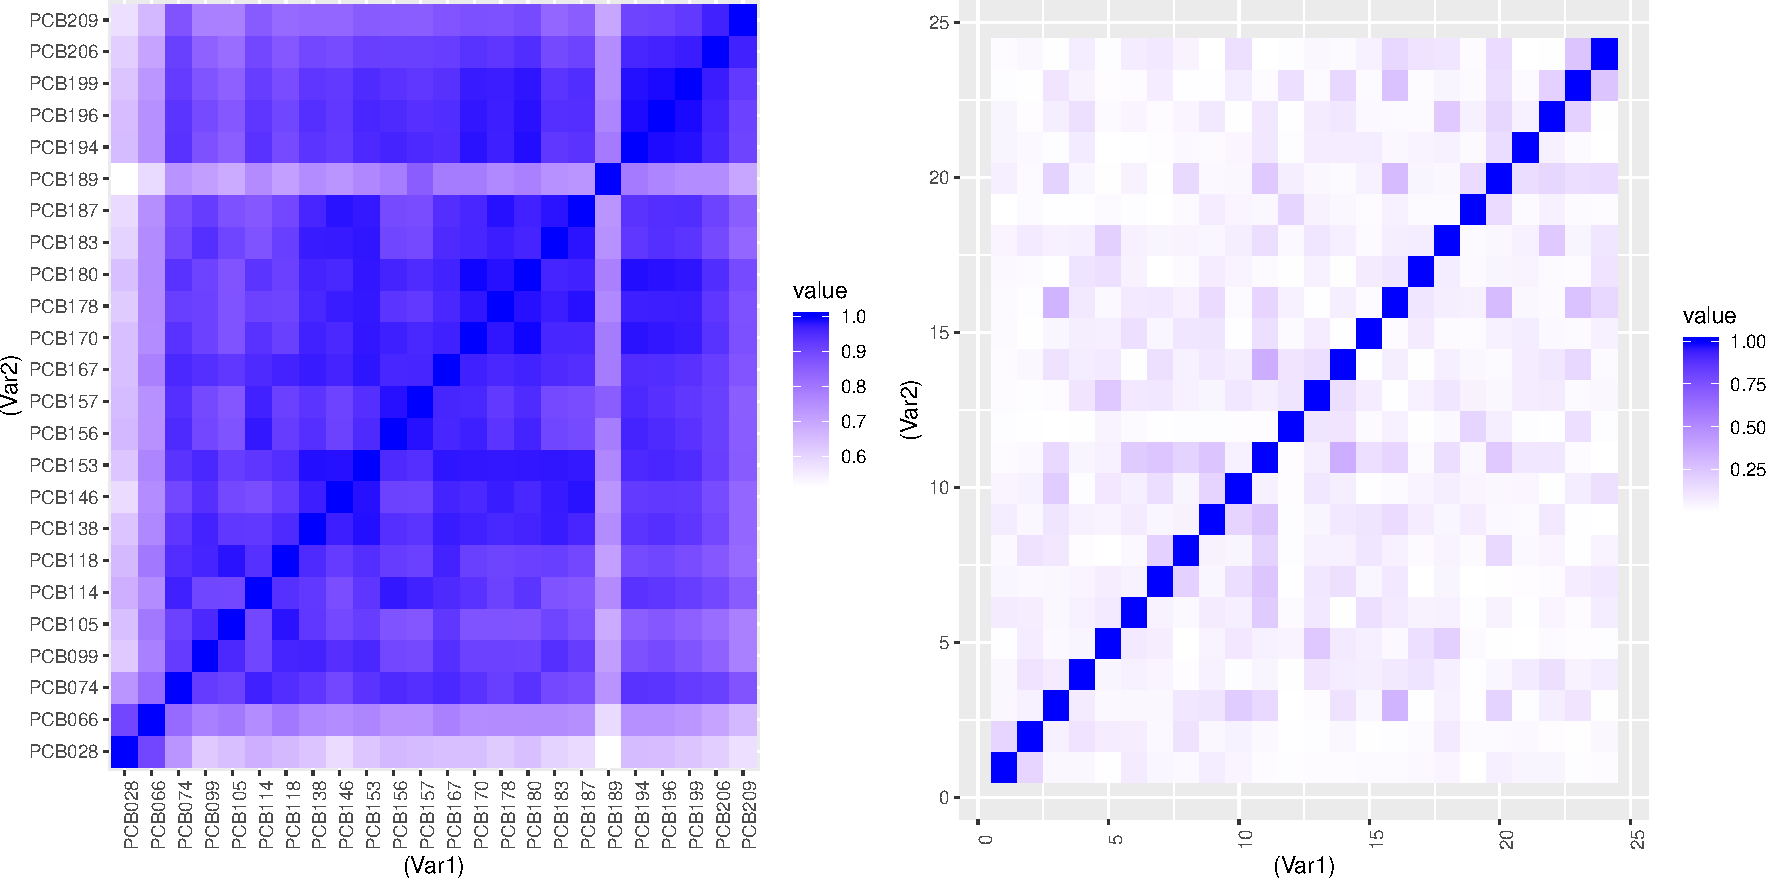
\includegraphics{PCBs_covariance_files/figure-latex/unnamed-chunk-31-1.pdf}
\caption{Female}
\end{figure}

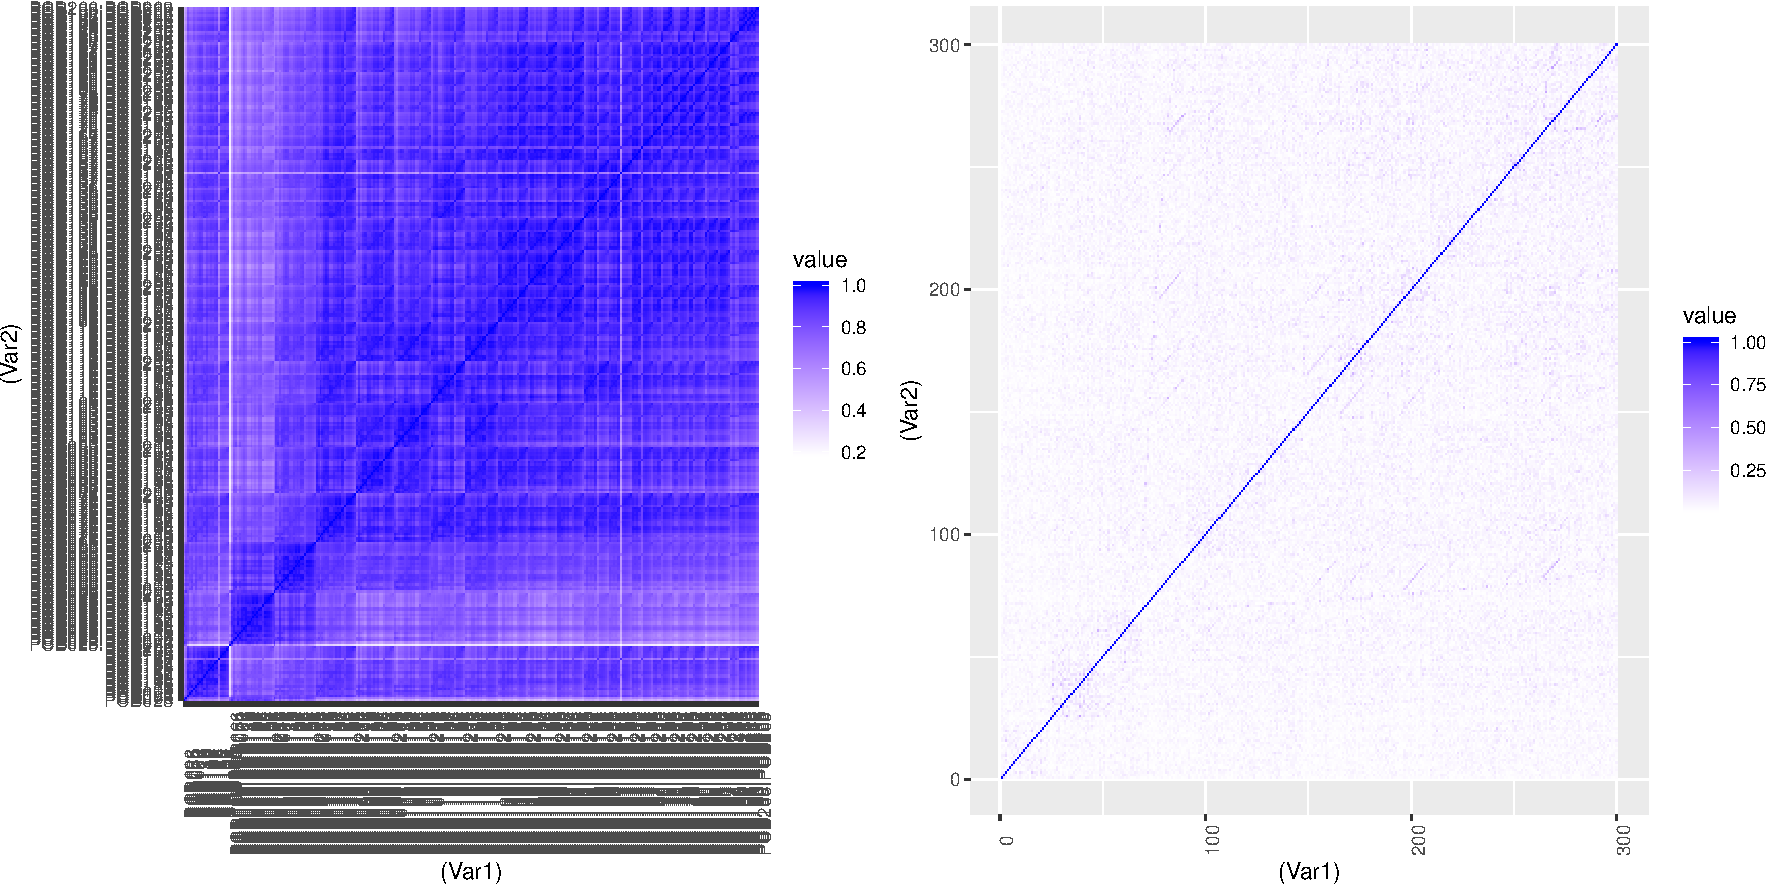
\includegraphics{PCBs_covariance_files/figure-latex/unnamed-chunk-32-1.pdf}


\end{document}
